% enable this to activate the version for PRINT
% disable this to make the pdf symmetric and without white pages
% => asymmetric alternating left/right margins
% \newcommand*{\printversion}{}%

%% | ---------------- document meta information --------------- |

\newcommand{\Author}{Yevhenii Kubov}
\newcommand{\Department}{Department of Cybernetics}
\newcommand{\Supervisor}{Ing. Matouš Vrba}
\newcommand{\SupervisorSpecialist}{Ing. My Specialist, Ph.D.}
\newcommand{\Programme}{Cybernetics and Robotics}
\newcommand{\Field}{TODO}
\newcommand{\Title}{Implementation of a neural network \\[0.5em]for autonomous trail following}
\newcommand{\Keywords}{Unmanned Aerial Vehicles, Robotic Perception, Deep Learning, Convolutional Neural Networks}
\newcommand{\KlicovaSlova}{Bezpilotní Prostředky, Robotické Vnímání, Hluboké Učení, Konvoluční Neuronové Sítě}
\newcommand{\Year}{2022}
\newcommand{\Month}{May}
\newcommand{\Date}{\Month~\Year}
\newcommand{\Location}{Prague}

%% | ---------------------- configuration --------------------- |

% most of the configuration stuff happens here
%!TEX root = ../main.tex

%% | ----------------------- page setup ----------------------- |

% define documentclass based on the print/screen version of the document
\pdfoutput=1
\ifdefined\printversion
  \documentclass[a4paper,11pt,twoside,openright]{book}
\else
  \documentclass[a4paper,11pt,oneside]{book}
\fi

% define how "clearpage" works with the print/screen version of the document
\newcommand{\conditionalClearPage}{
  \ifdefined\printversion
    \cleardoublepage
  \else
    \clearpage
  \fi
}

%% | ----------------- commonly used packages ----------------- |

\usepackage[english]{babel}
\usepackage[utf8]{inputenc}
\usepackage{csquotes}
\usepackage{amsmath,amsfonts,amssymb,bm}
\usepackage{nicefrac}
\usepackage{algorithm,algpseudocode}
\usepackage[title,titletoc]{appendix}
\usepackage{latexsym}
\usepackage{a4wide}
\usepackage{color}
\usepackage{indentfirst}
\usepackage{graphicx}
\usepackage{fancyhdr,lastpage}
\usepackage{longtable}
\usepackage{pifont}
\usepackage{makeidx}
\usepackage{multirow}
\usepackage{dcolumn}
\usepackage{epstopdf}
\usepackage{url}
\usepackage{listings}
\usepackage{relsize}
\usepackage{pdfpages}
\usepackage{url}
\usepackage{lipsum}
\usepackage{isotope}
\usepackage{verbatim}
\usepackage{xcolor}
\usepackage{tcolorbox}
\usepackage[hidelinks]{hyperref}
\usepackage{multicol}
\usepackage{subfig}
\usepackage[export]{adjustbox}
\usepackage{gensymb}

% print version has different margins to accommodate the spine of the book
% do not move this around, or it stops working
\ifdefined\printversion
  \usepackage[a4paper,margin=3.2cm,inner=3.4cm,outer=2.0cm]{geometry}
\else
  \usepackage[a4paper,margin=3.2cm,inner=2.7cm,outer=2.7cm]{geometry}
\fi

\hyphenation{}

%% | ---------------------- abbreviations --------------------- |

\usepackage[printonlyused]{acronym}

% use to change margins around abbreviations block
\def\changemargin#1#2{\list{}{\rightmargin#2\leftmargin#1}\item[]}
\let\endchangemargin=\endlist

%% | -------------------------- tikz -------------------------- |

\usepackage{tikz}
\usepackage{pgfplots}
\pgfplotsset{compat=1.14}
\usetikzlibrary{backgrounds,arrows,automata,shapes,positioning,calc,through,spy,shapes,shapes.geometric,shapes.multipart,fit,patterns,fadings}
\pgfdeclarelayer{background}
\pgfdeclarelayer{foreground}
\pgfsetlayers{background,main,foreground}

%% | ------------ siunitx for units of measurements ----------- |

\usepackage{siunitx}
\DeclareSIUnit \parsec {pc}
\DeclareSIUnit \electronvolt {eV}
\DeclareSIUnit \pixel {px}
\DeclareSIUnit \arcmin {arcmin}
\DeclareSIUnit \erg {erg}
\DeclareSIUnit \joul {J}

%% | --------------- change formatting of lists --------------- |

\usepackage{enumitem}
\setlist{nosep}

%% | -------------------- table of contents ------------------- |

\usepackage[subfigure]{tocloft}

\tocloftpagestyle{plain}

%% | ----------------- formatting of a chapter ---------------- |

\usepackage{titlesec}
\titleformat{\chapter}[block]
{\normalfont\huge\bfseries}{Chapter \thechapter\\\vspace{0.1em}\\}{1em}{\Huge}
% {?}{before}{after}
\titlespacing*{\chapter}{0pt}{-1em}{2em}

%% | ------------------------ biblatex ------------------------ |

\usepackage[backend=bibtex,defernumbers=false,style=ieee,sorting=ydnt,sortcites=true]{biblatex}

%% DEFERNUMBERS WAS CHANGED TO FALSE FROM TRUE

% define the source file with bibliography
\addbibresource{main.bib}

\renewcommand*{\bibfont}{\Font}

% add suffix "a" to publications containing the keyword "mine"
% add suffix "c" to publications containing the keyword "mine" && "core"
\DeclareFieldFormat{labelnumber}{%
  \ifkeyword{mine}
    {\ifkeyword{core}
      {{\number\numexpr#1}c}%
      {{\number\numexpr#1}a}%
    }%
    {#1}%
}

\DeclareCiteCommand{\tabcite}%[\mkbibbrackets]
  {\usebibmacro{cite:init}%
   \usebibmacro{prenote}}
  {\usebibmacro{citeindex}%
   \usebibmacro{cite:comp}}
  {}
  {\usebibmacro{cite:dump}%
   \usebibmacro{postnote}}

% define fullciteinbox command
\definecolor{light-gray}{gray}{0.95}
\newcommand{\fullciteinbox}[2]{%

\DeclareCiteCommand{\fullcite}
{\usebibmacro{prenote}}
{\clearfield{addendum}%
  \usedriver
  {\defcounter{minnames}{6}%
  \defcounter{maxnames}{6}}
{\thefield{entrytype}}}
{\multicitedelim}
{\usebibmacro{postnote}}

\begin{tcolorbox}[width=\textwidth,colback={light-gray},title={}]%
\ifx&#2&
\else
  \textbf{#2}:\\\\
\fi
\begin{minipage}[t]{0.07\linewidth}%
\raggedright%
\cite{#1}%
\end{minipage}%
\begin{minipage}[t]{0.93\linewidth}%
\fullcite{#1}%
\end{minipage}%
\end{tcolorbox}%
%}%
\vspace{-0.3em}
}%

% change the bibliography font style
% does not compile without this
\let\bibfont\small

%% | ---------------------- custom macros --------------------- |

\newcommand{\strong}[1]{\textbf{#1}}
\newcommand{\coord}[1]{\textbf{#1}}
\newcommand{\norm}[1]{\left\lvert#1\right\rvert}
\newcommand{\m}[1]{\ensuremath{\mathbf{#1}}}
\newcommand\numberthis{\addtocounter{equation}{1}\tag{\theequation}}
\newcommand{\add}[1]{{\color{green} {#1}}}
\newcommand{\todo}[1]{{\color{red} TODO {#1}}}
\newcommand{\updated}[1]{{\color{blue} {#1}}}
\newcommand{\real}{\mathbb{R}}
\newcommand{\red}[1]{{\color{red} #1}}
\newcommand{\minus}{\scalebox{0.75}[1.0]{$-$}}
\newcommand{\plus}{\scalebox{0.8}[0.8]{$+$}}
\newcommand{\figvspace}{\vspace{-1em}}

% referencing
\newcommand{\reffig}[1]{Fig.~\ref{#1}}
\newcommand{\reflst}[1]{Lst.~\ref{#1}}
\newcommand{\refalg}[1]{Alg.~\ref{#1}}
\newcommand{\refsec}[1]{Sec.~\ref{#1}}
\newcommand{\reftab}[1]{Table~\ref{#1}}
\newcommand{\refeq}[1]{\eqref{#1}}

%% | ----------------- listings - showing code ---------------- |

\usepackage{listings}     
\usepackage{lstautogobble}  % Fix relative indenting
\usepackage{color}          % Code coloring
\usepackage{zi4}            % Nice font

\definecolor{bluekeywords}{rgb}{0.13, 0.13, 1}
\definecolor{greencomments}{rgb}{0, 0.5, 0}
\definecolor{redstrings}{rgb}{0.9, 0, 0}
\definecolor{graynumbers}{rgb}{0.5, 0.5, 0.5}

\usepackage{listings}
\lstset{
    autogobble,
    columns=fullflexible,
    showspaces=false,
    showtabs=false,
    breaklines=true,
    showstringspaces=false,
    breakatwhitespace=true,
    escapeinside={(*@}{@*)},
    commentstyle=\color{greencomments},
    keywordstyle=\color{bluekeywords},
    stringstyle=\color{redstrings},
    numberstyle=\color{graynumbers},
    basicstyle=\ttfamily\footnotesize,
    frame=l,
    framesep=12pt,
    xleftmargin=12pt,
    tabsize=4,
    captionpos=b
}

%% | -------------------- layout parameters ------------------- |

% no indent, free space between paragraphs
\setlength{\parindent}{1cm}
\setlength{\parskip}{1ex plus 0.5ex minus 0.2ex}

% offsets the head down
\setlength{\headheight}{18pt}

% foot line
\renewcommand{\footrulewidth}{0.4pt}

%% | -------------- define the 'full' page style -------------- |

\fancypagestyle{full}{%

  % clear the default layout
  \fancyhead{}
  \fancyfoot{}

  % page header
  \fancyhead[LO]{\leftmark}
  \fancyhead[RE]{\rightmark}
  \fancyhead[LE,RO]{\thepage/\pageref{LastPage}}

  % page footer
  \fancyfoot[L]{CTU in Prague}
  \fancyfoot[R]{\Department}
  \fancyfoot[C]{}
}

%% | -------------- define the 'plain' page style ------------- |

\fancypagestyle{plain}{%

  % clear the default layout
  \fancyhead{}
  \fancyfoot{}

  % page header
  \fancyhead[LE,RO]{\thepage}
}

%% | -------------- Adjust style of chapter names ------------- |

\renewcommand{\chaptermark}[1]{\markboth{\MakeUppercase{\thechapter.\ #1}}{}}

%% | -------- European layout, no extra space after '.' ------- |

\frenchspacing

%% | ----------- adjust the style of the first page ----------- |

\makeatletter
\renewcommand\chapter{\if@openright\cleardoublepage\else\clearpage\fi
                    \thispagestyle{full}% original style: plain
                    \global\@topnum\z@
                    \@afterindentfalse
                    \secdef\@chapter\@schapter}
\makeatother


%% | ---------------------- the contents ---------------------- |

\begin{document}

\pagenumbering{roman}

%% --------------------------------------------------------------
%% |                         Title page                         |
%% --------------------------------------------------------------

%!TEX root = ../main.tex

\begin{titlepage}
  \begin{center}

    \textsc{\Large Czech Technical University in Prague}\\[1em]
    \textsc{\large Faculty of Electrical Engineering\\
    \Department\\
    Multi-robot Systems\\[3em]
    }
    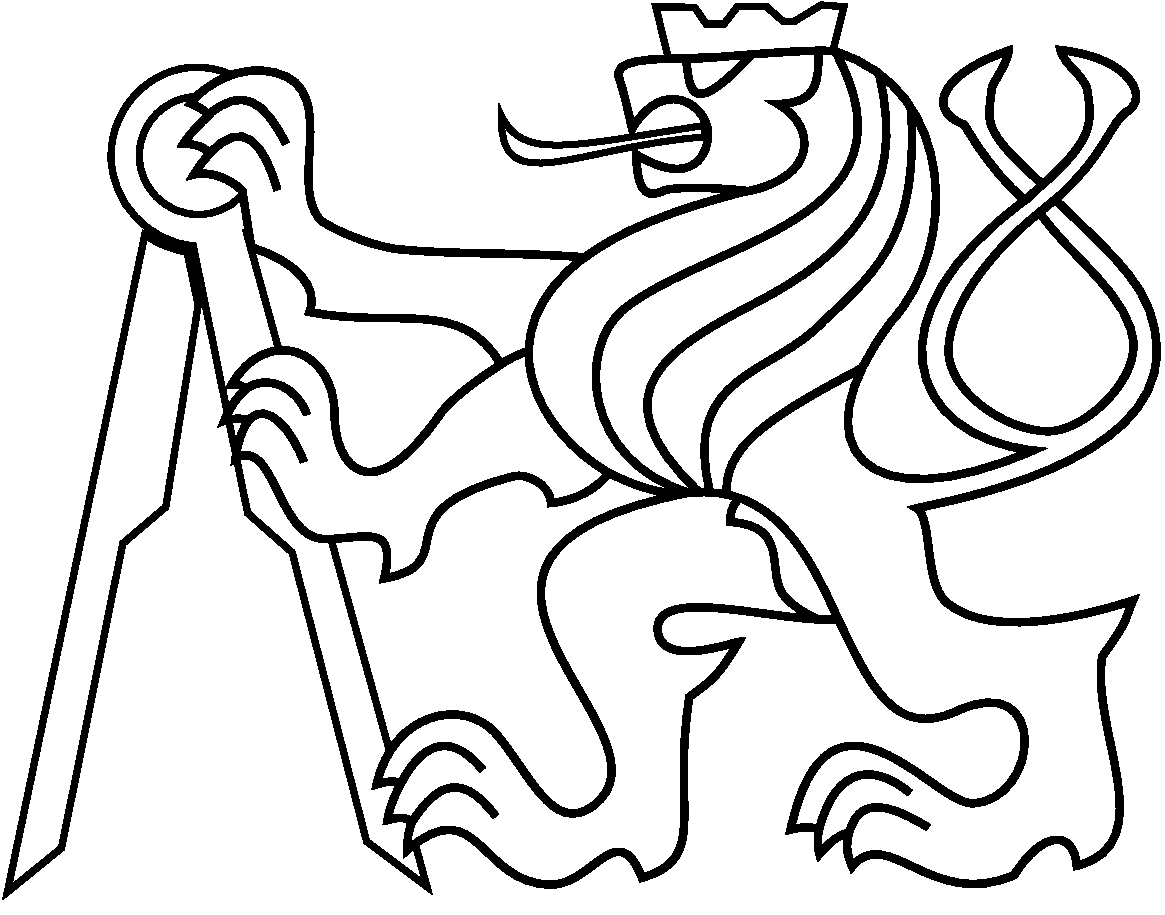
\includegraphics[height=4.1cm]{fig/ctu_lion.pdf}\\[3em]

    \textbf{\textsc{\Huge \Title}}\\[2em]

    \textbf{\Large Bachelor's Thesis}\\[6em]

    \textbf{\huge \Author}\\[6em]

    {\large \Location, \Date}\\[3em]

    Study programme: \Programme\\[6em]
    %Branch of study: \Field\\[4em]

    \textbf{Supervisor: \Supervisor}\\

    \vspace{2pt}

  \end{center}
\end{titlepage}


% set up the page style for the "intro" pages
\pagestyle{plain}

%% --------------------------------------------------------------
%% |                       Acknowledgments                      |
%% --------------------------------------------------------------

\conditionalClearPage

%!TEX root = ../main.tex

\section*{Acknowledgments}

Firstly, I would like to express my gratitude to my supervisor.

\vspace{2.5cm}


%% --------------------------------------------------------------
%% |                         Assignment                         |
%% --------------------------------------------------------------

\conditionalClearPage

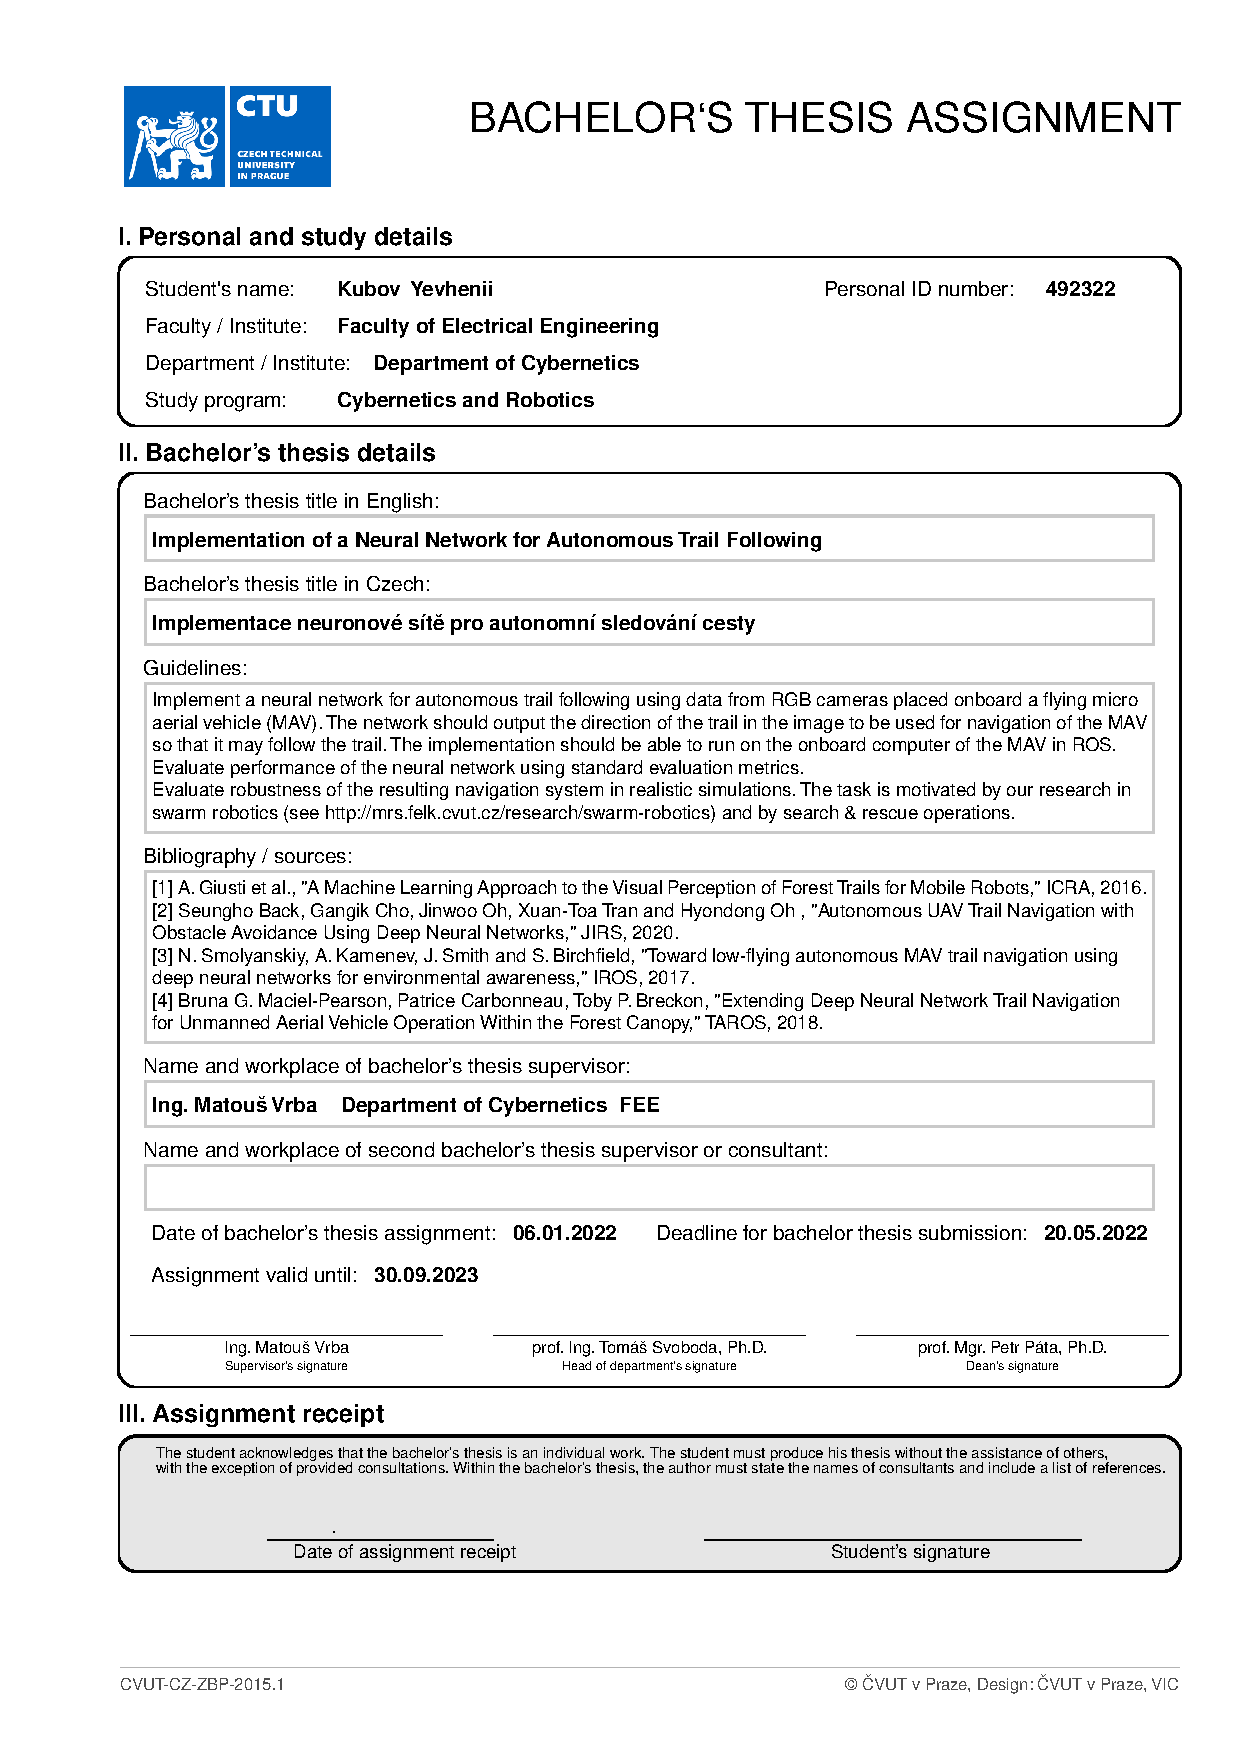
\includepdf{src/assignment.pdf}

%% --------------------------------------------------------------
%% |                          Abstracts                         |
%% --------------------------------------------------------------

\conditionalClearPage

%!TEX root = ../main.tex

\begin{changemargin}{0.8cm}{0.8cm}

~\vfill{}

\section*{Abstract}
\vskip 0.5em

The problem of autonomously following a trail by a robot based on images from an onboard monocular camera is tackled in this thesis. A robotic system that solves the task of flying through a forest along a man-made dirt trail is presented. It is accomplished by using a classification deep convolutional neural network for determining in which direction relative to the trail is the camera pointing. The output of this classifier is then used to command the robot to follow the trail. It was implemented to run online onboard an MRS multi-rotor micro aerial vehicle. Part of the implementation is also an algorithm for path planner trajectory generation. Performance and robustness was tested in simulations, followed by real-world experiments. The implemented system showed good practical results and can be used as a starting point for more complex navigation and surveillance applications.

\vskip 1em

{\bf Keywords} \Keywords

\vskip 2.5cm

\end{changemargin}


\conditionalClearPage

%!TEX root = ../main.tex

\begin{changemargin}{0.8cm}{0.8cm}

~\vfill{}

\section*{Abstrakt}
\vskip 0.5em

\sloppy
Tato práce je zaměřená na problematiku sledování lesní cesty pomocí obrázku z monokulární kamery, připevněné na bezpilotní helikoptéře nebo pozemním vozidle. Je představen systém, řešící úlohu navigace podél stezky v lese. Toho bylo dosaženo s využitím klasifikační hluboké konvoluční neuronové sítě pro určení směru natočení helikoptéry vzhledem k cestě. Systém byl implementován s minimálním zpožděním, aby mohl být zapojen ve zpětné vazbě s plánováním trajektorie helikoptéry v rámci MRS UAV systému. Součastí implementace je algoritmus na generování bodů trajektorie pro plánovač. Výkon a robustnost byly otestovány v simulaci a následně během experimentů v reálném světe. Implementovaný systém prokázal dobré praktické výsledky a může být použit jako výchozí bod pro komplexnější navigační a průzkumné aplikace.

\vskip 1em

{\bf Klíčová slova} \KlicovaSlova

\vskip 2.5cm

\end{changemargin}


%% --------------------------------------------------------------
%% |                        Abbreviations                       |
%% --------------------------------------------------------------

\conditionalClearPage

\begin{changemargin}{0.8cm}{0.8cm}

~\vfill{}

\section*{Abbreviations}

% this will print only the used abbreviations
%!TEX root = ../main.tex

\begin{acronym}
  \acro{CTU}[CTU]{Czech Technical University}
  \acro{FOV}[FOV]{Field of View}
  \acro{GNSS}[GNSS]{Global Navigation Satellite System}
  \acro{GPS}[GPS]{Global Positioning System}
  \acro{IMU}[IMU]{Inertial Measurement Unit}
  \acro{LiDAR}[LiDAR]{Light Detection and Ranging}
  \acro{MAV}[MAV]{Micro Aerial Vehicle}
  \acro{MRS}[MRS]{Multi-robot Systems Group}
  \acro{ROS}[ROS]{Robot Operating System}
  \acro{UAV}[UAV]{Unmanned Aerial Vehicle}
  \acro{UGV}[UGV]{Unmanned Ground Vehicle}
  \acro{RGB}[RGB]{Red Green Blue additive colour model}
  \acro{USB}[USB]{Universal Serial Bus}
  \acro{IR}[IR]{Infrared}
  \acro{CNN}[CNN]{Convolutional Neural Network}
  \acro{DNN}[DNN]{Deep Neural Network}
  \acro{SAR}[SAR]{Search and Rescue}
  \acro{GPU}[GPU]{Graphics Processing Unit}
\end{acronym}


\vskip 2.5cm

\end{changemargin}

\conditionalClearPage

%% --------------------------------------------------------------
%% |                      Table of contents                     |
%% --------------------------------------------------------------

\tableofcontents

\conditionalClearPage

% set up the full page style with normal page numbering
\pagestyle{full}
\pagenumbering{arabic}


\chapter{Introduction}


\section{Unmanned Aerial Vehicles}
Flying robots, also called \acs{UAV}s have been used since the first half of the 20th century \cite{keane2013brief}. They were still controlled by a human operator, but allowed for dangerous tasks to be performed remotely, like aerial target practices. Originally designed for military purposes, they evolved into a vast industry. Since that time, electronic hardware has become much more compact, power-efficient, cheap and advanced. Also, aircraft designs have strongly evolved after decades of research, battery power improved, software got advanced as never before. Nowadays, all those factors allow for a wide usage of compact and relatively inexpensive vehicles in many industries and research. 

\acs{UAV}s can be equipped with different payloads and sensors, depending on their task (\reffig{fig:firefighter}). For example, thermal cameras are used for border control, detecting animals in wildlife, or forest fires. \acs{LiDAR}s can be used for 3D mapping of the area, for navigation in obstructed environment. Digital cameras are good for crops analysis, area mapping, surveillance, monitoring of different constructions or power lines. 


\begin{figure}[!h]
  \centering
  \includegraphics[width=0.6\textwidth]{./fig/photos/firefighter.jpeg}

  \caption{\acs{MRS} \acs{MAV} equipped with firefighting and thermal imaging modules.}
  \label{fig:firefighter}
\end{figure}


\acs{UAV}s are also important for \ac{SAR} missions. Benefits of using them in such operations is that these vehicles are usually portable, have small deployment time and generally require only minimal qualification to operate them, thanks to flight computers with advanced software. They can be used instead of human teams, reducing the risk for their life or health in dangerous environments. \acs{UAV}s may be also cheaper than alternatives, especially manned aircraft, and faster than rescue teams or ground vehicles. They are usually not only less expensive, but also provide data logging from all sensors, including \acs{GPS} and associated image data from high resolution cameras. This data can be used even for later review. For \acs{SAR} missions usually two types of \acs{UAV}s are used: fixed-wing aircraft and multi-rotor helicopters. First ones provide higher speed, flight time, but are less agile and take longer time to take off and land the vehicle. Multi-rotors have the ability to hover, fly close to the ground, in buildings, caves and other complex terrains. In this thesis, a multi-rotor \acs{MAV} will be used as an airframe. 


\section{Convolutional neural networks}

Neural networks (also called artificial neural networks) are algorithms, whose design was inspired by biological neural networks in human and animal brains. Their structure consists of nodes called neurons, and connections between them. Every connection has its weight. Neurons are grouped into layers, each layer has its unique number of them. Neurons which receive value (stimuli) on input from outside of the network are input neurons. Those who receive values from other neurons, process this data and output the result to other neurons are hidden neurons. Those who output the result outside the network are called output neurons. Mentioned weights of connections between neurons can be adjusted through the learning process. During it, a network learns to identify needed shapes in the input and produce a correct decision according to the task. 

Convolutional neural networks have been experiencing tremendous growth during the last 10 years, allowing for many previously unsolved problems to be tackled \cite{li2021survey}. They are used in military, healthcare, aerospace, social media, science and other applications. This approach allowed for faster and more accurate analysis of many diseases even on early stages, using measurements performed on the patient, which are then fed to a neural network. In aerospace and automotive engineering neural networks are often used as component fault detectors and for improved guidance systems. In electronics their capabilities help to expose failures when producing the chips, synthesise voice, compress data and solve many other tasks. In military they help to identify hostile objects or enemies. 


There are different types of neural networks. Several examples are presented in this chapter.

\subsection{Segmentation networks}
Among the most popular types are segmentation neural networks. Their goal is to divide an image into multiple segments. In such architecture, each pixel refers to some class or object type. This type is often used for biomedical applications. Good example is U-Net architecture, frequently used in light microscopy \cite{ronneberger2015u}.

\subsection{Recurrent networks}

This type of networks is used for problems, such as language translation and speech recognition. They are designed to handle sequential data on input (\reffig{fig:recurrent}).

\begin{figure}[!h]
  \centering
  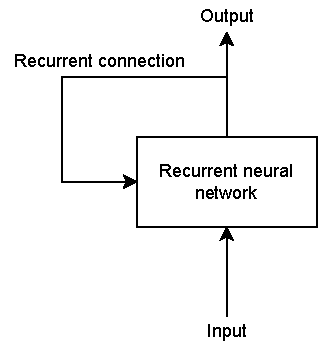
\includegraphics[width=0.5\textwidth]{./fig/photos/recurrent.pdf}

  \caption{Example of a recurrent network architecture.}
  \label{fig:recurrent}
\end{figure}

\subsection{Generative adversarial networks}

GAN networks consist of two neural networks, that contest with each other. Each network's gain is another network's loss. One network called discriminator identifies how much the input image is "realistic", while other (generator) generates this input and adjusts it to "fool" the discriminator.

\subsection{Classification networks}

One of the most popular are classification neural networks. In such use-case given an input image, a neural network must identify to which class does an image belong. Good example is Alexnet architecture for classification on 1000 classes subset from the ImageNet dataset \cite{krizhevsky2012imagenet}. Back in 2012 it won the ImageNet large-scale visual recognition challenge. This type of a neural network is used in this thesis. Architecture is from \cite{giusti2016machine}.

\section{Trail following}

In this thesis, the problem of trail following using image from monocular camera onboard a multi-rotor \acs{MAV} is tackled, including the implementation of a working algorithm, solving the task. Following the man-made forest path is natural for humans, because it is usually the most efficient way to get through this complex terrain. Such policy, in most cases, minimises the travel time and possible injury to a person (\reffig{fig:challenging_path}). The same applies to robots. Human paths are freely passable, unlike random trajectories in a forest, and it is a reason to stay on them.

\begin{figure}[!h]
  \centering
  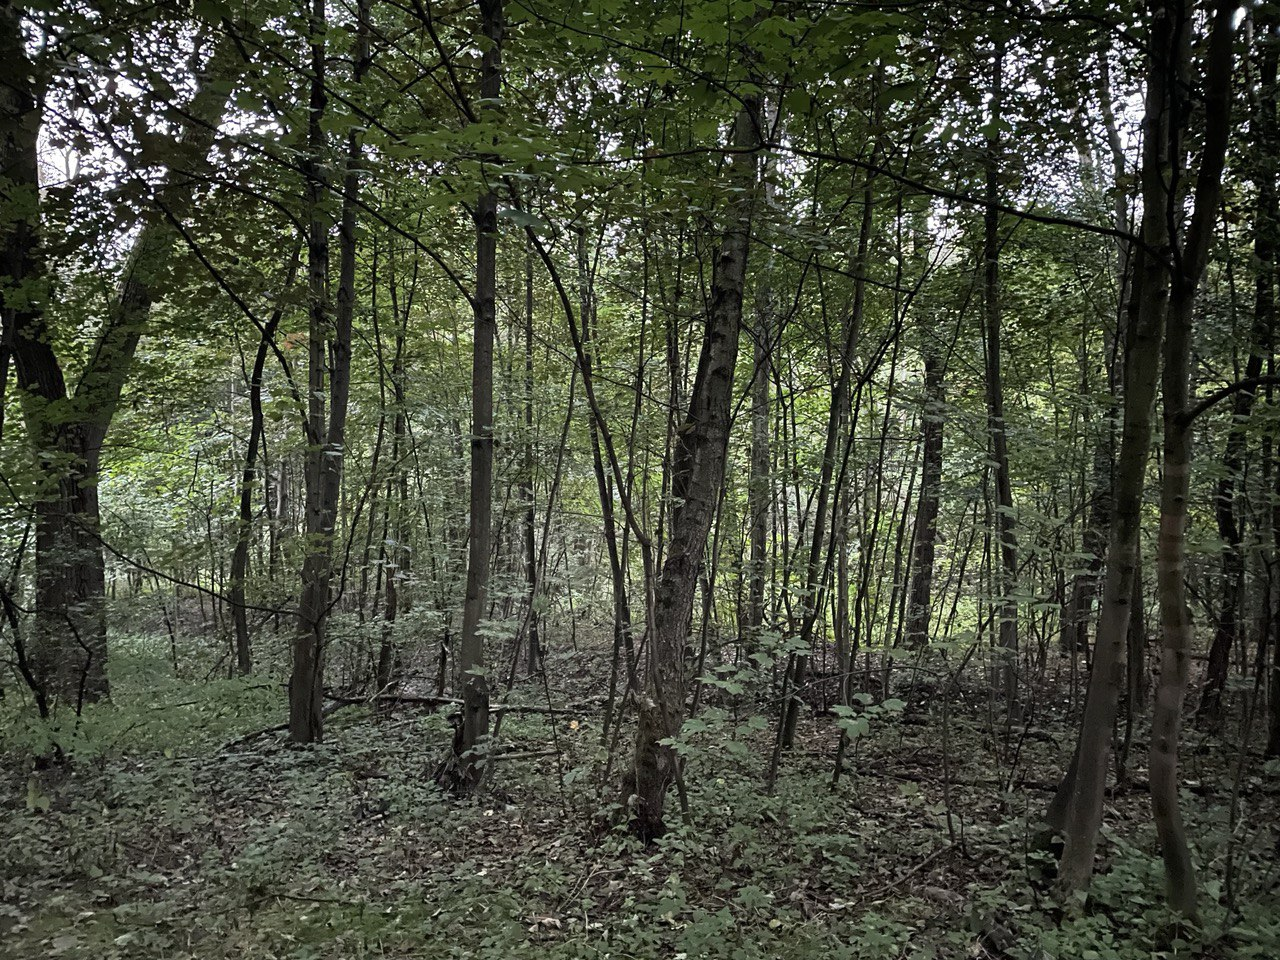
\includegraphics[width=0.75\textwidth]{./fig/photos/challenging_path.jpg}

  \caption{Random path in a forest is generally challenging to pass.}
  \label{fig:challenging_path}
\end{figure}

Trail following is an important task for autonomous navigation of robots. Suggested use-cases are search and rescue missions, efficient navigation through forests and mapping of the area. Motivation for this task is a situation when there is no opportunity to communicate with and control the vehicle manually or when an autonomous mission is highly preferred. The goal is to allow for a quadcopter or unmanned ground vehicle (UGV) to navigate through a forest using computer vision techniques. Having the image from the onboard camera, the vehicle should determine which direction to travel when flying through a forest, utilising the trail. It must strictly follow the human path.

Algorithms solving related problems like lane-following, lane-departure and lane-assist for cars on public roads, were introduced in 1990's \cite{batavia1999driver} and are commonly used in personal vehicles since the early 2000's \cite{chen2020lane}. But there is a clear distinction between the lane on a road and a forest trail. In the first case, the lane is marked with contrast symbols and lines, making the task solvable by simple segmentation algorithms, based on in-image contrast and colour variance, image saliency \cite{santana2013tracking}. Forest trail images provide smaller amount of distinguishable features (\reffig{fig:features_difference}) and it may be challenging even for humans to determine the direction of travel \cite{giusti2016machine}.

\begin{figure}[!h]
  \centering
  \subfloat[Image of a trail from the dataset \cite{giusti2016machine}.] {
    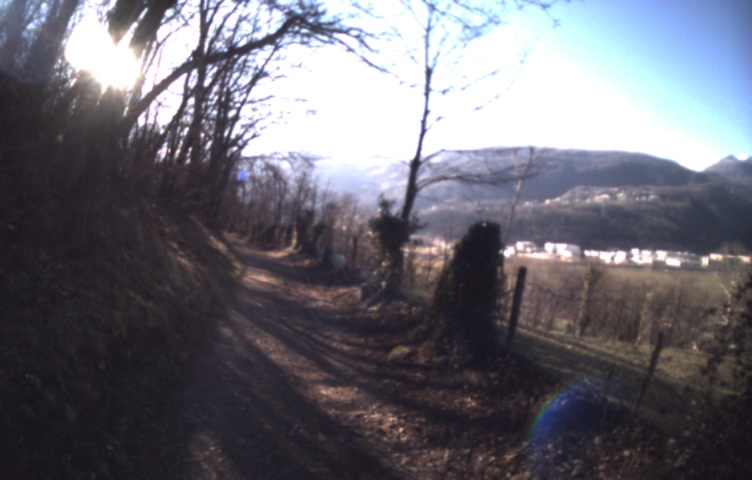
\includegraphics[width=0.48\textwidth]{./fig/photos/trail1.jpg}
    \label{fig:trail_1}
  }
  \subfloat[Image of a road taken by myself.] {
    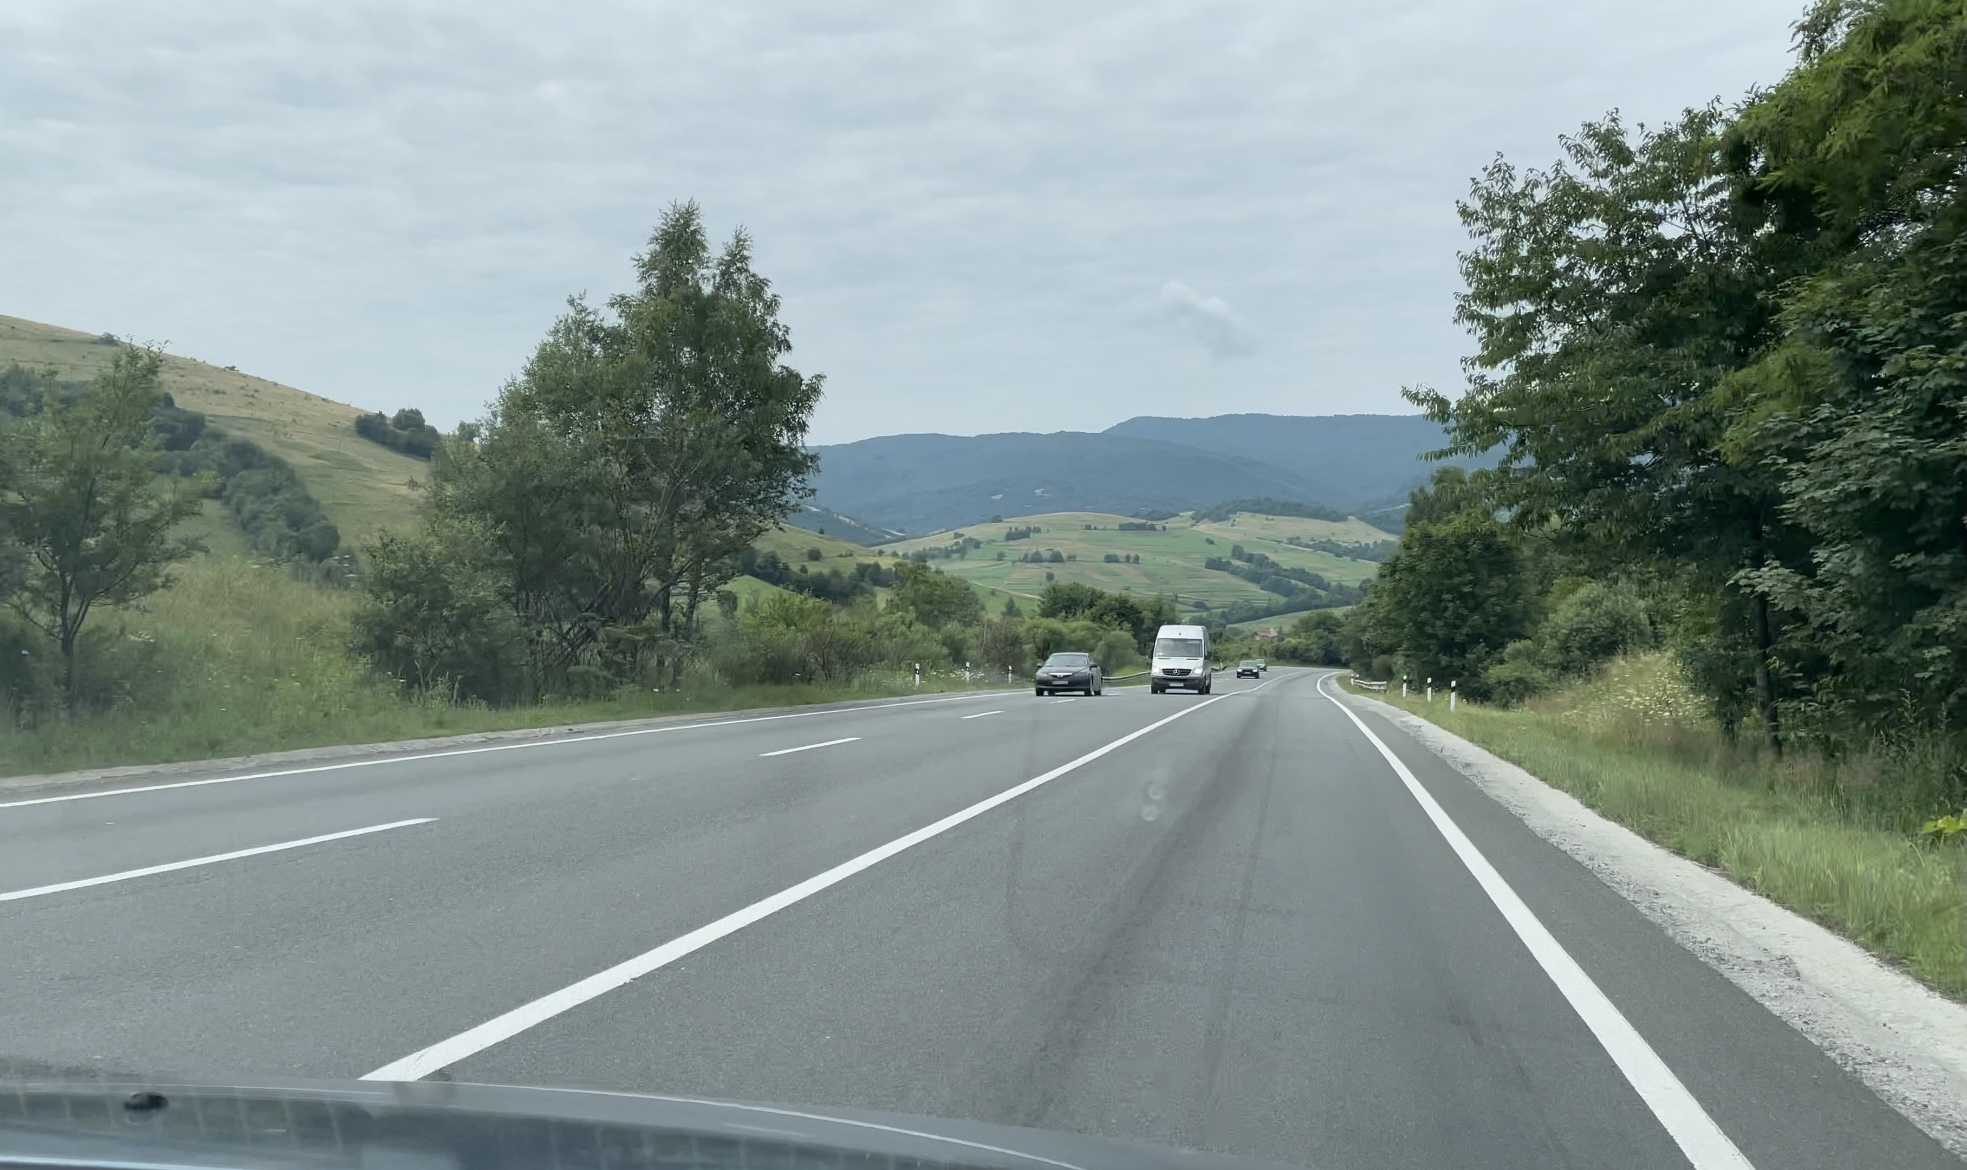
\includegraphics[width=0.48\textwidth]{./fig/photos/road.PNG}
    \label{fig:road_1}
  }
  \caption{Difference between a forest trail on \reffig{fig:trail_1} and a road on \reffig{fig:road_1}.}
  \label{fig:features_difference}
\end{figure}


One of the first effectively solved by neural networks, but still topical problems is classification. Neural networks are able to learn and then identify features, corresponding to pre-defined classes, and combinations of those features \cite{krizhevsky2012imagenet}. This makes it possible to effectively classify, which class an image belongs to. 

Treating the trail following task as a classification problem is a different approach that specifically tackles it. For this approach classes like "Left", "Right" and "Straight" can be introduced \cite{giusti2016machine}. It allows to estimate the current direction of a vehicle, given the probabilities of these classes and to plan the trajectory of the \acs{MAV} accordingly. 


\begin{figure}[!h]
  \begin{minipage}{.5\linewidth}
  \centering
  \subfloat[Class "left".] {
    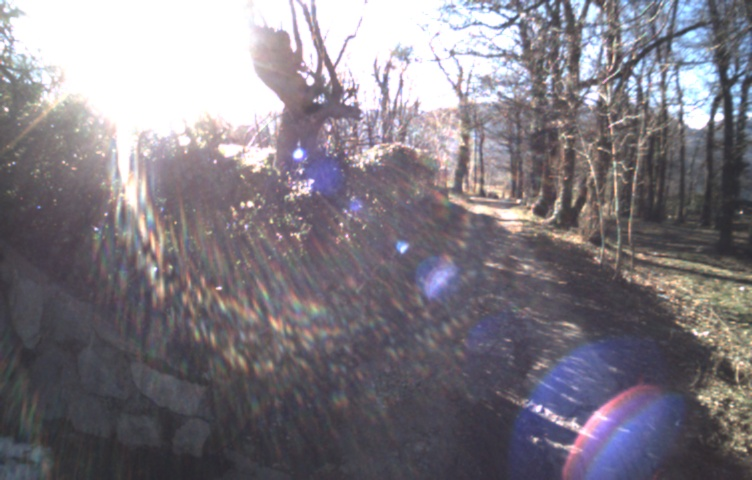
\includegraphics[width=0.95\textwidth]{./fig/photos/class_l.jpg}
    \label{fig:class_l}
  }
  \end{minipage}
  \begin{minipage}{.5\linewidth}
  \centering	
  

  \subfloat[Class "right".] {
    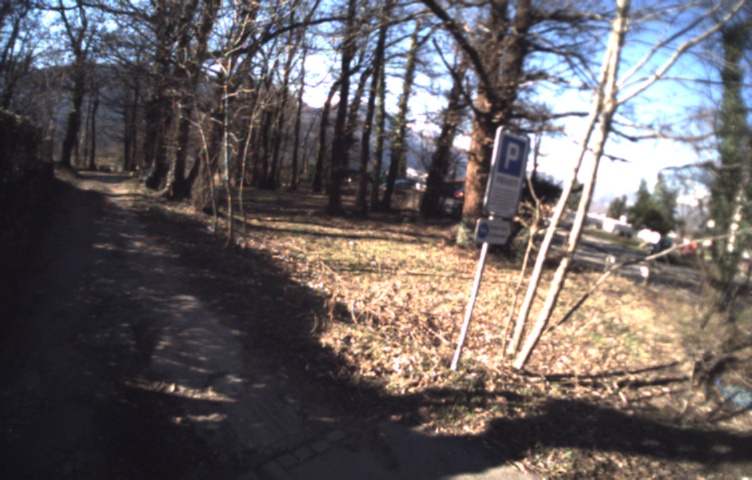
\includegraphics[width=0.95\textwidth]{./fig/photos/class_r.jpg}
    \label{fig:class_s}
  }
  \end{minipage}\par\medskip
  \centering
  \subfloat[Class "straight".] {
    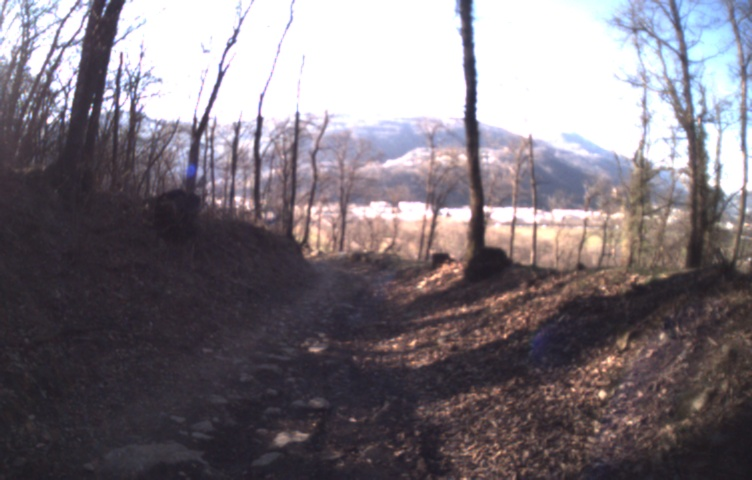
\includegraphics[width=0.5\textwidth]{./fig/photos/class_s.jpg}
    \label{fig:class_r}
  }
  \caption{Example images of different classes}
  \label{fig:classes}
\end{figure}

This thesis focuses on implementation of the trail-following algorithm using classification convolutional neural network. The implementation should run online in the Gazebo simulation environment as well as onboard a \acs{MAV} in a real-world deployment. Therefore, delay of the algorithm must be sufficiently small. The task is to design an algorithm that autonomously provides a \acs{MAV} with a relatively safe direction and speed of movement. The \acs{MAV} is equipped with PX4 flight computer, Intel NUC companion computer, and Intel RealSense camera. The environment may contain obstacles, but is assumed that the trail is obstacle-free. 

Implemented neural network can be used as an entry point for more sophisticated surveillance and navigation algorithms. For more complex environments a possible enhancement is usage alongside with obstacle avoidance algorithms and lateral correction \cite{back2020autonomous, maciel2018extending, smolyanskiy2017toward}.















\chapter{Methodology}

TODO: Is backpropagation description good enough? (and formulas?)

In this thesis an architecture suggested by \citeauthor{giusti2016machine} will be used. It consists of 4 convolutional layers, each followed by hyperbolic tangent activation and max pooling layer, and then a fully connected layer with 200 hidden neurons. Network processes images from a camera, attached to a vehicle. Input layer is formed by $3\times 101\times101$ neurons. Therefore, input \acs{RGB} image must be anisotropically resized to a size $101\times101$ pixels to be fed directly to the network. After going through all the hidden layers and the softmax output layer it produces 3 probabilities of each class, which sum to 1. Based on these probabilities it is possible to determine at which direction is the camera most probably pointed. Given the fact that side cameras are pointed $30 \degree$ from the centre, interpolation is also possible based on these probabilities.  


\section{\acs{CNN}}
\subsection{Convolutions}

Convolution is a fundamental mathematical operation used in a wide range of image processing techniques. In the context of Convolutional Neural Networks, convolution of an input matrix $I$ with a so called "kernel" matrix $K$ is applied to obtain an output matrix $O$. The kernel is typically smaller and is applied to submatrices of $I$ to extract features corresponding to $K$ in different regions of $I$. The convolutional layer of a \acs{CNN} typically also contains a bias term $w_0$. The kernel matrix $K$ and the bias $w_0$ are parameters that are learned during the training phase using the backpropagation algorithm, described in section \ref{backprop}. 
\begin{equation}
	\begin{bmatrix}
    x_{11}       & x_{12} & x_{13} & \dots & x_{1n} \\
    x_{21}       & x_{22} & x_{23} & \dots & x_{2n} \\
    \hdotsfor{5} \\
    x_{r1}       & x_{r2} & x_{r3} & \dots & x_{rn}
\end{bmatrix}\,,
\label{Input data}
\end{equation}

\begin{equation}
	\begin{bmatrix}
    w_{11}       & w_{12} & w_{13} \\
    w_{21}       & w_{22} & w_{23} \\
    w_{31}       & w_{32} & w_{33} 
	\end{bmatrix}\,.
\label{Kernel}
\end{equation}

Convolution is performed by "stamping" a kernel onto input data, starting from the upper left angle, and thus creating a linear combination of input array members and kernel weights. Let the input data be \eqref{Input data} and convolutional kernel be \eqref{Kernel}. Then, the result of the first application of convolution kernel will be:

\begin{equation}
\begin{aligned}
	O(1, 1) = x_{11}\cdot w_{11} + x_{12}\cdot w_{12} + x_{13}\cdot w_{13} +\\
	x_{21}\cdot w_{21} + x_{22}\cdot w_{22} + x_{23}\cdot w_{23} + \\
	x_{31}\cdot w_{31} + x_{32}\cdot w_{32} + x_{33}\cdot w_{33} + w_0\,.
\end{aligned}
\end{equation}

And the equation for convolutional kernel stamp starting on i-th row and j-th column of the input image (where the convolution is defined) is:

\begin{equation}
	O(i, j) = w_0 + \sum\limits_{k=1}^m \sum\limits_{l=1}^n I_{i+k-1, j+l-1}\cdot K_{k, l} \,,
\end{equation}
where kernel has $m$ rows and $n$ columns, $i$ runs from 1 to $M-m+1$, $j$ runs from 1 to $N-n+1$. Kernel is $K$, input image is $I$. To produce the output array, filter must slide through the whole input image.


\subsection{Hyperbolic tangent}

For neural network to not act as a linear classifier, a nonlinearity should be introduced in its hidden layers. It allows the network to solve more complex tasks and increase its performance. It is also a nature-inspired approach. Nonlinearity is introduced using nonlinear activation layers, added after each convolutional layer. Most popular activation functions are Rectified Linear Unit (ReLU), Leaky ReLU, Sigmoid and Hyperbolic Tangent. The last one is used in this thesis. Hyperbolic Tangent has very similar shape to the Sigmoid and also maps the output only to the range of [-1, 1] (\reffig{fig:htangent}). It is calculated using the following equation:
\begin{equation}
	\textrm{tanh}(x) = \frac{e^x-e^{-x}}{e^x+e^{-x}}\,,
\end{equation}
where $x$ is the real input value obtained after convolution stamp.

\begin{figure}[!h]
  \centering
  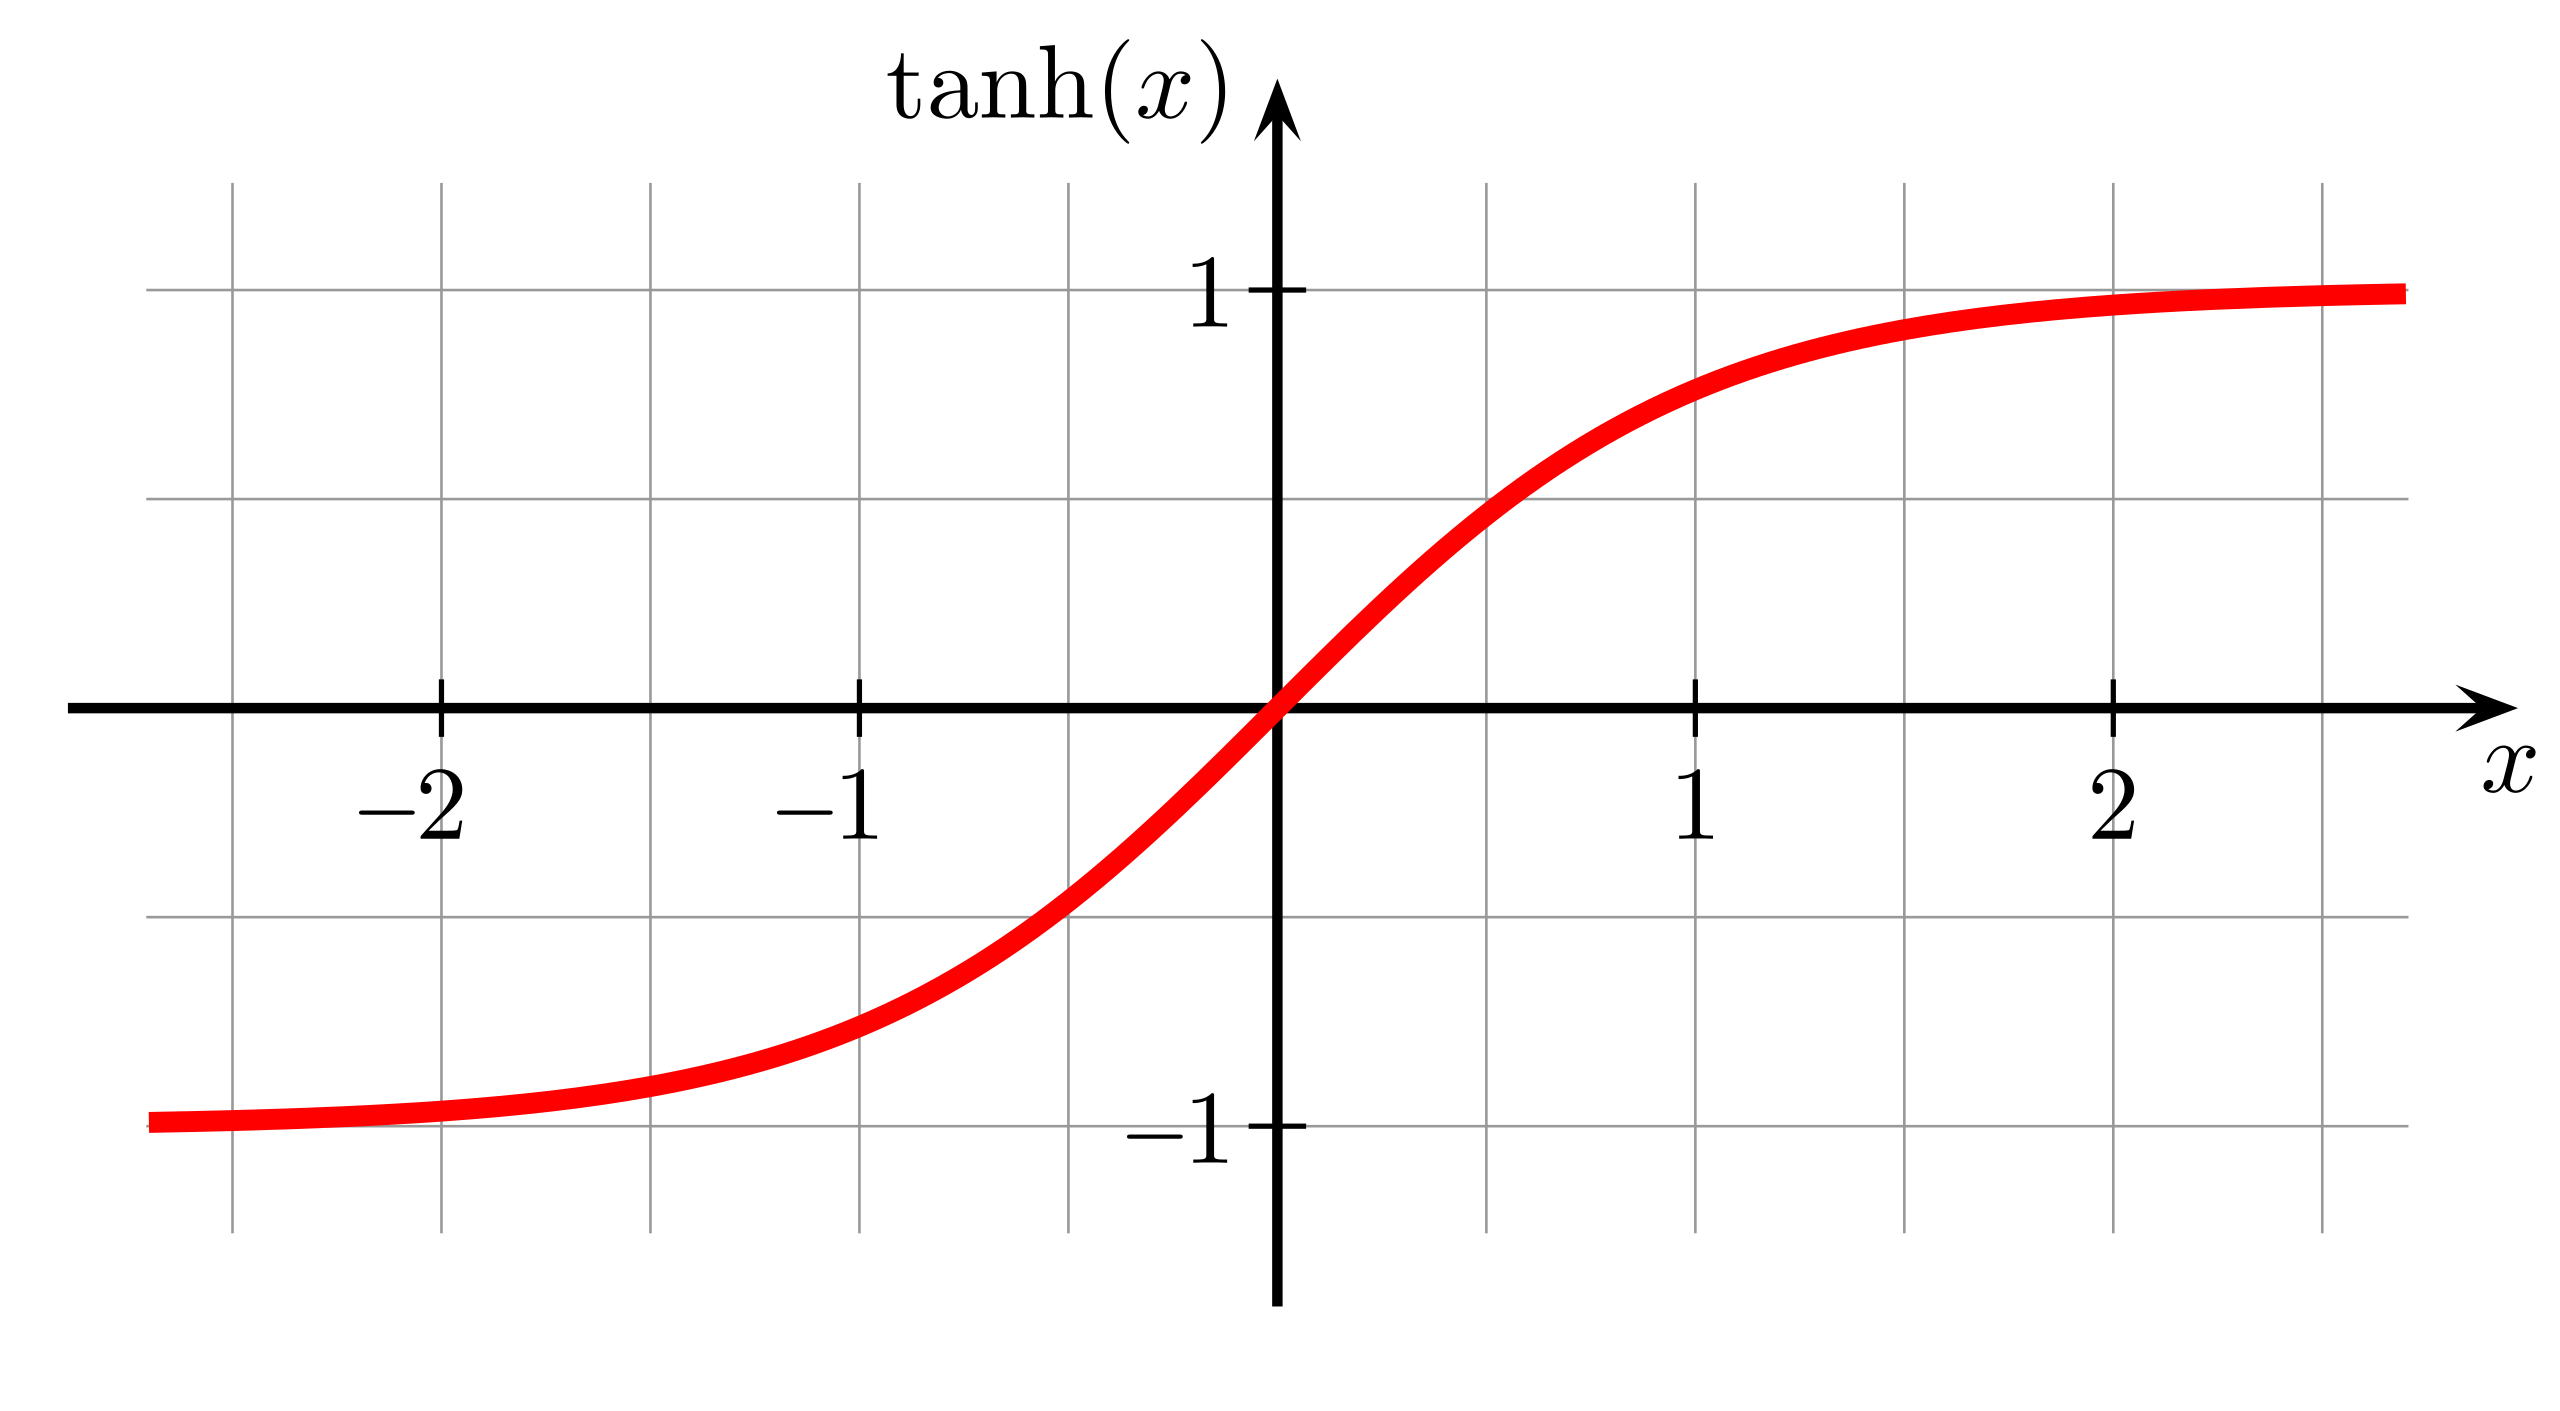
\includegraphics[width=0.6\textwidth]{./fig/photos/hyperbolic_tangent.png}

  \caption{Hyperbolic Tangent function.}
  Author: Geek3, CC BY-SA 3.0, https://commons.wikimedia.org/w/index.php?curid=4198479
  \label{fig:htangent}
\end{figure}


\subsection{Max-pooling}

Max-pooling is an operation, applied to some part of the input data array, taking only the maximum value of this area. It is typically used in the form of a rectangular filter, which slides through the whole image. It produces only one output value from each filter-sized input area, thus can be used for downsampling of the image, taking only the most significant values to the output. In this way, the learning process of the neural network is sped up because the amount of learnable weights is decreased. Also, better resistance to distortions and affine transformations is obtained \cite{yu2014mixed}.

\subsection{Softmax}

Softmax is widely used in neural network architectures as the last layer. It has same amount of outputs as inputs. Softmax function may have any real values on input, including positive, negative, zero, but its output values are always in the range $[0, 1]$ and they always sum to 1. These properties allow the output to be in form of "probabilities" of each corresponding input value. This layer normalises the output, which is from $\textrm{R}^n$ to probability distribution.

The softmax function is defined as:

\begin{equation}
	\sigma(\vec z)_i = \frac{e^{z_i}}{\sum\limits_{j=1}^n e^{z_j}}\,,
\end{equation}
where $z_i$ are elements of the real input vector, $\sigma(\vec z)$ is output vector, $n$ is the number of outputs.


\begin{figure}[!h]
  \centering
  
  \documentclass{standalone}
\usepackage{pgfplots}
\usepackage{bm}
\usepackage{siunitx}
\pgfplotsset{compat=1.12}
\usetikzlibrary{arrows, decorations.pathmorphing, backgrounds, positioning,fit,petri}
\usetikzlibrary{calc}

\newcommand{\xdistl}{6cm}
\newcommand{\xdistr}{4cm}

\begin{document}

\begin{tikzpicture}
  \fontsize{11}{11}
  {
    \node[black, draw, thick, rounded corners] (f1) at (0, 0) {Input image 101x101x3};
    \node[black, draw, thick, rounded corners] (f2) [below=of f1] {Feature map 98x98x32};
    \node[black, draw, thick, rounded corners] (f3) [below=of f2] {Feature map 49x49x32};
    \node[black, draw, thick, rounded corners] (f4) [below=of f3] {Feature map 46x46x32};
    \node[black, draw, thick, rounded corners] (f5) [below=of f4] {Feature map 23x23x32};
    \node[black, draw, thick, rounded corners] (f6) [below=of f5] {Feature map 20x20x32};
    \node[black, draw, thick, rounded corners] (f7) [below=of f6] {Feature map 10x10x32};
    \node[black, draw, thick, rounded corners] (f8) [below=of f7] {Feature map 8x8x32};
    \node[black, draw, thick, rounded corners] (f9) [below=of f8] {Feature map 4x4x32};
    \node[black, draw, thick, rounded corners] (f10) [below=of f9] {200 hidden neurons};
    \node[black, draw, thick, rounded corners] (f11) [below=of f10] {3 neurons};



    \draw[->, line width=2pt] (f1.south) -| (f2.north);
    \draw[->, line width=2pt] (f2.south) -| (f3.north);
    \draw[->, line width=2pt] (f3.south) -| (f4.north);
    \draw[->, line width=2pt] (f4.south) -| (f5.north);
    \draw[->, line width=2pt] (f5.south) -| (f6.north);
    \draw[->, line width=2pt] (f6.south) -| (f7.north);
    \draw[->, line width=2pt] (f7.south) -| (f8.north);
    \draw[->, line width=2pt] (f8.south) -| (f9.north);
    \draw[->, line width=2pt] (f9.south) -| (f10.north);
    \draw[->, line width=2pt] (f10.south) -| (f11.north);



    \node[black, draw, opacity=0, text opacity=1, anchor=west] (l1) at ( $ (f1)!0.5!(f2) + (2, 0)$ ) {Convolution, 4x4 kernel, 1 stride, no padding, tanh activation};
    \node[black, draw, opacity=0, text opacity=1, anchor=west] (l2) at ( $ (f2)!0.5!(f3) + (2, 0)$ ) {Max-pooling, 2x2 kernel, 2 stride, no padding};
    \node[black, draw, opacity=0, text opacity=1, anchor=west] (l3) at ( $ (f3)!0.5!(f4) + (2, 0)$ ) {Convolution, 4x4 kernel, 1 stride, no padding, tanh activation};
    \node[black, draw, opacity=0, text opacity=1, anchor=west] (l4) at ( $ (f4)!0.5!(f5) + (2, 0)$ ) {Max-pooling, 2x2 kernel, 2 stride, no padding};
    \node[black, draw, opacity=0, text opacity=1, anchor=west] (l5) at ( $ (f5)!0.5!(f6) + (2, 0)$ ) {Convolution, 4x4 kernel, 1 stride, no padding, tanh activation};
    \node[black, draw, opacity=0, text opacity=1, anchor=west] (l6) at ( $ (f6)!0.5!(f7) + (2, 0)$ ) {Max-pooling, 2x2 kernel, 2 stride, no padding};
    \node[black, draw, opacity=0, text opacity=1, anchor=west] (l7) at ( $ (f7)!0.5!(f8) + (2, 0)$ ) {Convolution, 4x4 kernel, 1 stride, 1 padding, tanh activation};
    \node[black, draw, opacity=0, text opacity=1, anchor=west] (l8) at ( $ (f8)!0.5!(f9) + (2, 0)$ ) {Max-pooling, 2x2 kernel, 2 stride, no padding};
    \node[black, draw, opacity=0, text opacity=1, anchor=west] (l9) at ( $ (f9)!0.5!(f10) + (2, 0)$ ) {Fully connected layer};
    \node[black, draw, opacity=0, text opacity=1, anchor=west] (l10) at ( $ (f10)!0.5!(f11) + (2, 0)$ ) {Output};



    \node[black, draw, opacity=0, text opacity=1, anchor=west] (ll1) at ( $ (f1)!0.5!(f2) - (3, 0)$ ) {Layer 1};
    \node[black, draw, opacity=0, text opacity=1, anchor=west] (ll2) at ( $ (f2)!0.5!(f3) - (3, 0)$ ) {Layer 2};
    \node[black, draw, opacity=0, text opacity=1, anchor=west] (ll3) at ( $ (f3)!0.5!(f4) - (3, 0)$ ) {Layer 3};
    \node[black, draw, opacity=0, text opacity=1, anchor=west] (ll4) at ( $ (f4)!0.5!(f5) - (3, 0)$ ) {Layer 4};
    \node[black, draw, opacity=0, text opacity=1, anchor=west] (ll5) at ( $ (f5)!0.5!(f6) - (3, 0)$ ) {Layer 5};
    \node[black, draw, opacity=0, text opacity=1, anchor=west] (ll6) at ( $ (f6)!0.5!(f7) - (3, 0)$ ) {Layer 6};
    \node[black, draw, opacity=0, text opacity=1, anchor=west] (ll7) at ( $ (f7)!0.5!(f8) - (3, 0)$ ) {Layer 7};
    \node[black, draw, opacity=0, text opacity=1, anchor=west] (ll8) at ( $ (f8)!0.5!(f9) - (3, 0)$ ) {Layer 8};
    \node[black, draw, opacity=0, text opacity=1, anchor=west] (ll9) at ( $ (f9)!0.5!(f10) - (3, 0)$ ) {Layer 9};
    \node[black, draw, opacity=0, text opacity=1, anchor=west] (ll10) at ( $ (f10)!0.5!(f11) - (3, 0)$ ) {Layer 10};

}
\end{tikzpicture}

\end{document} 

  
  \caption{Used neural network architecture.}
  \label{fig:architecture}
\end{figure}


% Input ^ adds 600 words, idk why


\section{Backward propagation of error}
\label{backprop}

Backward propagation is the way to calculate the gradient of the loss function $\frac{\partial J}{\partial \textbf{w}}$ with respect to the vector of weights $\textbf{w}$\,. Calculated gradient has the same length as weights vector. It means how much each weight affects and contributes to the value of the loss function. This knowledge is used to change the weights in a way that minimises the loss. 

First part of backpropagation is a forward pass. Given the input data and the weights, output of the neural network is calculated and compared with ground truth through the loss function. Then, backward pass starts. Partial derivatives are calculated sequentially through each layer, starting from the last one, and after multiplication give the total gradient $\frac{\partial J}{\partial \textbf{w}}$\,.

Used in this thesis architecture consists of convolutional layers, max-pooling layers, hyperbolic tangent activation and fully connected layers. Max-pooling chooses one input with the maximum value and feeds it directly to the output, other inputs are ignored. It doesn't have learnable parameters affecting the gradient. In convolutional layer back propagation is the convolution of input feature map with the upstream gradient. Derivative of hyperbolic tangent is $\frac{d\textrm{tanh}(x)}{dx} = 1-\textrm{tanh}(x)^2$.



\section{Loss function}

To successfully train the neural network, a loss function is necessary. It estimates the "penalty" of the difference between a ground truth and prediction of the neural network. Loss function outputs one real value based on this data. Then, using the back propagation, a "penalty" gets minimised. In this thesis I use a cross-entropy loss criterion. Its equation is:

\begin{equation}
	Loss = -\sum\limits_{x=0}^n p(x)\cdot \textrm{log} \,q(x) \,,
\end{equation}
where $n$ is the number of classes, $p(x)$ is the desired probability of the class (ground truth), $q(x)$ is the prediction from the neural network.




\chapter{Implementation}

TODO: system image/scheme

\section{System hardware}

\subsection{Pixhawk flight controller}

Pixhawk is a low-cost advanced flight computer with open-source hardware. There are different variations of form factors, featuring different amount of input/output ports. Pixhawk is very flexible in terms of attachable peripherals, stable and well-tested. Most essential sensors like accelerometers, gyro, digital compass (magnetometer) and barometer are already part of the main board. \acs{MRS} vehicles have these boards flashed with open-source PX4 autopilot software. Features like advanced regulators, estimators, interface for controlling the \acs{UAV} and others are already implemented in this software, usually only minor tweaking is needed. Thus an abstraction from the \acs{MAV} hardware is created, allowing the vehicle to be controlled using high-level commands.


\subsection{Intel NUC companion computer}

NUC is a compact high-performance, yet power-efficient computer, capable of running demanding AI and machine learning software. It is possible to install the whole \acs{MRS} system on it, including \acs{ROS} software to command trajectories, speed and other parameters to a flight controller and act as a main high-level computational unit. \acs{ROS} is run inside Ubuntu operating system on this board, so other software can be used simultaneously. Different peripherals can be connected to a computer via \acs{USB}. For this thesis a RealSense camera is connected, from which my algorithm (written in Python programming language) is receiving images for processing.

\subsection{Intel RealSense D435 camera}

D435 is a powerful camera capable of taking normal \acs{RGB} pictures as well as depth images. It has a wide \acs{FOV}, which is perfect for robotic applications. Also its stereo imagers feature global shutter, which is important in low-light conditions or during fast movements. The camera consists of 4 modules: right imager, \acs{IR} projector, left imager and \acs{RGB} module. However, for this thesis only the \acs{RGB} module will be used. Its sensor has a resolution of 2\,MP and produces $1920\times1080$ images at the frame rate of 30 frames per second.


\section{Used software tools}

\subsection{Python}

I have chosen the Python programming language for this task. It is a high-level language with simple syntax, that features high user-readability and supports object-oriented approach. It is dynamically-typed and offers garbage collection feature. Thanks to these properties, it is considered to be one of the easiest programming languages to use. However, algorithms, written purely in Python are usually inefficient compared to the same ones written in low-level languages. But on the other hand, it has a lot of available powerful frameworks, especially for machine learning and neural networks, which are internally implemented in faster low-level languages like C++. So, the speed reduction will not be critical in this case. In this thesis a relatively powerful onboard PC is used, a bit slower code is not a problem. But in a situation where the fastest possible execution time is needed, another language should be considered. 

\subsection{PyTorch framework}

PyTorch is a powerful open-source machine learning framework for Python. It is often used for computer vision tasks, contains many pre-implemented modules and features, which makes it usable in a wide variety of applications and for most neural network types. It is actively developed and maintained. Framework is written in Python, C++ and CUDA languages, but Python is used mainly as an interface for it. Low-level operations are not implemented in Python due to its relative slowness. PyTorch is capable of running on \acs{GPU} to accelerate tensor computing, however, CUDA-capable Nvidia \acs{GPU} must be used. 


\section{Dataset}

For this task, I have chosen dataset from the authors of \acs{CNN} architecture \cite{giusti2016machine}, but any similar dataset can be used. Requirement is that every image must be labeled to one of the three classes. Used dataset was acquired by a hiker, wearing three head-mounted cameras: one pointing straight ahead, one pointing 30 degrees left, one pointing 30 degrees right. Originally images were labeled corresponding to the expected action: images from the camera pointed to the left are of class "turn right" (TR), from the forward camera are of class "go straight" (GS), from the right camera are of class turn "left" (TL) (see \reffig{fig:classes}).

However, I decided to change the classes definition to be more intuitive: in my code, there will be classes LEFT (for the camera pointed 30 degrees left), STRAIGHT (forward camera), and RIGHT (for the camera pointed 30 degrees right). Dataset is divided in such a way that approximately 75\% of it is used for training, and 25\% for validation. So, the neural network estimates the current direction relative to the trail, and based on this knowledge, further decision can be made.

\section{Neural network code}

The neural network is trained for 90 epochs, with a batch size of 512, but even larger size should be considered if the GPU has enough memory. Adam optimizer is used, with an initial learning rate of 0.005. Also, a scheduler is set, for reducing the learning rate by 5\% on each epoch. The criterion for training is the cross-entropy loss. 

\subsection{Training algorithm}

After the initialization of the neural network model, optimizer, scheduler, and criterion, the program enters a 90-epoch loop. In each epoch the data loaders are created for training and validation, each receives its part of the data from the pickle file, where the whole prepared dataset is stored. Then starts the training part where the forward pass and the back-propagation are calculated, optimizer step is done. After that validation part begins and the scheduler step is performed. In the end, after sufficient amount of iterations the weights of the neural network are saved for further usage.

\section{Program for preparing the dataset}

The downloaded dataset was structured into 14 folders (sub-parts), each containing folders “lc” (left camera), “rc” (right camera), “sc”(straight-pointing camera). Inside each one, there is a folder with the name ending “.frames”. Images from it must be moved one level up and the “.frames” folder must be deleted. 

Inside the code, a user must set the path to the dataset, select whether preparation of training or validation part is needed, and specify the range of sub-parts to be used (for example, 1-9 for training and 10-14 for validation).

For each selected sub-part program iterates through all images from the dataset, performs transformations so that the images correspond to the required format. In this case, they are resized to 101 by 101 pixels. Then it appends the transformed image to the data array and its label to the label array. After that, these arrays are saved to the python dictionary under fields ‘data’ and ‘label’. In the end, this dictionary is saved to the pickle .pkl file as “trn.pkl” or “val.pkl”, according to the choice of part in the previous paragraph.

Pickle is a tool for serialization of Python objects, which is handy in this case, because the whole prepared, ready-to-use dataset can be transferred as a single file.

\section{Navigation algorithm}

Two different approaches were tested in this thesis. First is angular and forward velocity generation, second is trajectory generation. 

\subsection{Velocity generation}

Generating velocities is the most intuitive way to utilise the neural network for trail following. In this case, input to a vehicle are only two values: angular velocity for heading correction and forward velocity for moving along the path when it is safe according to neural network outputs. Angular velocity $\omega$ can be calculated using a simple formula:

\begin{equation}
	\omega = (\textrm{p}(x = \textrm{R}) - \textrm{p}(x = \textrm{L}))\cdot\omega_{max}\,,
\end{equation}
where $\textrm{p}(x = \textrm{R})$ is the probability of the current direction being "right", $\textrm{p}(x = \textrm{L})$ is the probability of the current direction being "left", $\omega_{max}$ is the maximum desired angular velocity. Forward speed $v_x$ is calculated according to a formula:

\begin{equation}
	v_x = \textrm{p}(x = \textrm{S})\cdot v_{max}\,,
\end{equation}
where $\textrm{p}(x = \textrm{S})$ is the probability of the current direction being "straight" and $v_{max}$ is the maximum desired longtitudinal velocity.


\subsection{Trajectory generation}

\acs{MRS} \acs{ROS}-based system allows to control a \acs{UAV} using trajectories. They are represented as a sequence of geometric poses, which a vehicle should take. Implemented neural network does not allow to predict future direction of travel and gives an output only for current position. Therefore, it is possible to predict only one point of the trajectory on every image pass through the neural network. This point can be immediately sent to a path planner. Such approach has a big advantage: the algorithm can be run simultaneously with obstacle avoidance and other features. Path planner can then decide whether suggested direction is safe or other maneuver must be taken to evade a collision.

A point is given to the system in a format of \texttt{Reference} \acs{MRS} message. It consists of a \texttt{float64} value "heading" and a \texttt{Point} message "position", formed by three \texttt{float64} values for the position in x, y and z axes. Therefore, each point is described by 4 \texttt{float} values. These points can be represented relative to the \acs{UAV} current position with tilt-correction (xy plane is always parallel to the ground and z is always perpendicular). 

Heading $\alpha$ for the trajectory point is calculated according to the formula:

\begin{equation}
	\alpha = (\textrm{p}(x = \textrm{R}) - \textrm{p}(x = \textrm{L}))\cdot \alpha_{max}\,,
\end{equation}
where $\alpha_{max}$ is the maximum desired increment in radians. Step in x-axis $r_x$ relative to the current position is calculated as

\begin{equation}
	r_x = \textrm{p}(x = \textrm{S})\cdot \textrm{cos}(\alpha)\cdot r_{max}\,,
\end{equation}
where $r_{max}$ is a maximum desired step length. Step in y-axis $r_y$ is calculated as
\begin{equation}
	r_y = \textrm{p}(x = \textrm{S})\cdot \textrm{sin}(\alpha)\cdot r_{max}\,.
\end{equation}
Altitude is considered to remain constant so for each point it is set to $(1.8 - actual\_height)$\,m above the ground. Similar altitude was used in the dataset. Parameters $\alpha_{max}$, $r_{max}$ can be calibrated for better performance.

Such policy will be used during the experiments because the ability to combine the algorithm with a path planner is a priority.

\subsection{Filtering of the neural network output}

Implemented neural network produces results online, at 30\,hz. During the operation, a lens flare or other short-term disturbance can occur. It leads to rapid changes in prediction and combined with trajectory generation creates wrong, potentially unsafe points in a trajectory. Therefore, output must be filtered. To get rid of high frequency changes, a low-pass filter must be used. In this thesis was decided to use a simple yet effective low pass filter: a moving average filter. For frame number $n$ it also remembers $k-1$ previous predictions and outputs average of these $k$ predictions. Value $k=15$ showed good results during tests and thus was used in this work.


\chapter{Simulation}

%TODO: Describe how to install and run the simulation.

%TODO: Describe how do I get data from the drone and then send commands.

\section{Software}

For simulation of such complex application a dedicated software is needed. The main tool for simulation and further usage in a real robot is Robot Operating System (ROS). It is a framework for robotic applications which offers abstraction from hardware, and even contains already implemented functions for communication between vehicles, sensors, cameras and other used hardware, both real and virtual. 
The communication is performed using high-level messages. For every hardware unit a node is created. These nodes can subscribe (receive information) or publish to some topic. Topic represents a virtual pipe, through which the information is transferred. For example, there is a program running on robot PC. Program is subscribed to the topic \texttt{"/image"}, where the image is obtained from the node \texttt{"/camera"} and receives image from it. Then, it processes the image, makes some decision after it and commands the speed using \texttt{"/speed"} topic of the node \texttt{"/drone"}. Usually there are topics also for trajectory, odometry and other features.

TODO: IMAGES OF ROS NODES AND TOPICS

Another tool used for simulation is Gazebo. It offers real-time graphical visualisation of the ongoing experiment. Very realistic scenarios can be created in this simulator, its engine allows for shaders, different lighting conditions, and even physics simulation. Therefore, a virtual model of the use-case scene and conditions is usually designed, including the vehicle itself. Such model makes it possible to conveniently test designed software before proceeding to real-world experiments as the cost of a mistake in the real world can be high. 

\section{Simulation setup}

For trail following simulation I decided to use the \acs{MRS} pre-configured setup for one-vehicle simulation (available at \href{https://github.com/ctu-mrs/simulation}{\acs{MRS} GitHub}). In my case I will run the system inside the singularity container. Default simulation does not include the onboard camera. Thus the \newline \texttt{enable\_mobius\_camera\_front} parameter was added to the startup config \texttt{session.yml}. I selected the "Baylands" world for simulation, because it has a section of forest path in it. 

The code must be also modified to be run in simulation. Only needed change is the topic, from which the images are received.

To start the simulation I run the script \texttt{start.sh} and wait for initialisation of all windows. Then in tmux I can switch to the free window where no process is currently running and there startup my python code. 

\section{Simulation results}

During the experiment in simulation, performance of the implemented algorithm was tested in close to real-world conditions. \acs{UAV} successfully managed to follow the trail without getting lost. There are some oscillations during the heading correction, but they can be removed by using more complex heading regulation and fine tuning. Overall performance is good and proposed methods for navigation along the path worked as expected. Vehicle stayed on trail for as long as simulation was going, without fails. However, used map is relatively simple and has no obstacles or confusing factors, it was used to check the basic performance. Further and more detailed testing is conducted in real-world conditions.


\begin{figure}[!h]

  \centering
  \subfloat[Neural network predicts that \acs{UAV} is most likely pointed right relative to the path, when it is actually pointed right. Vehicle turns left.] {
    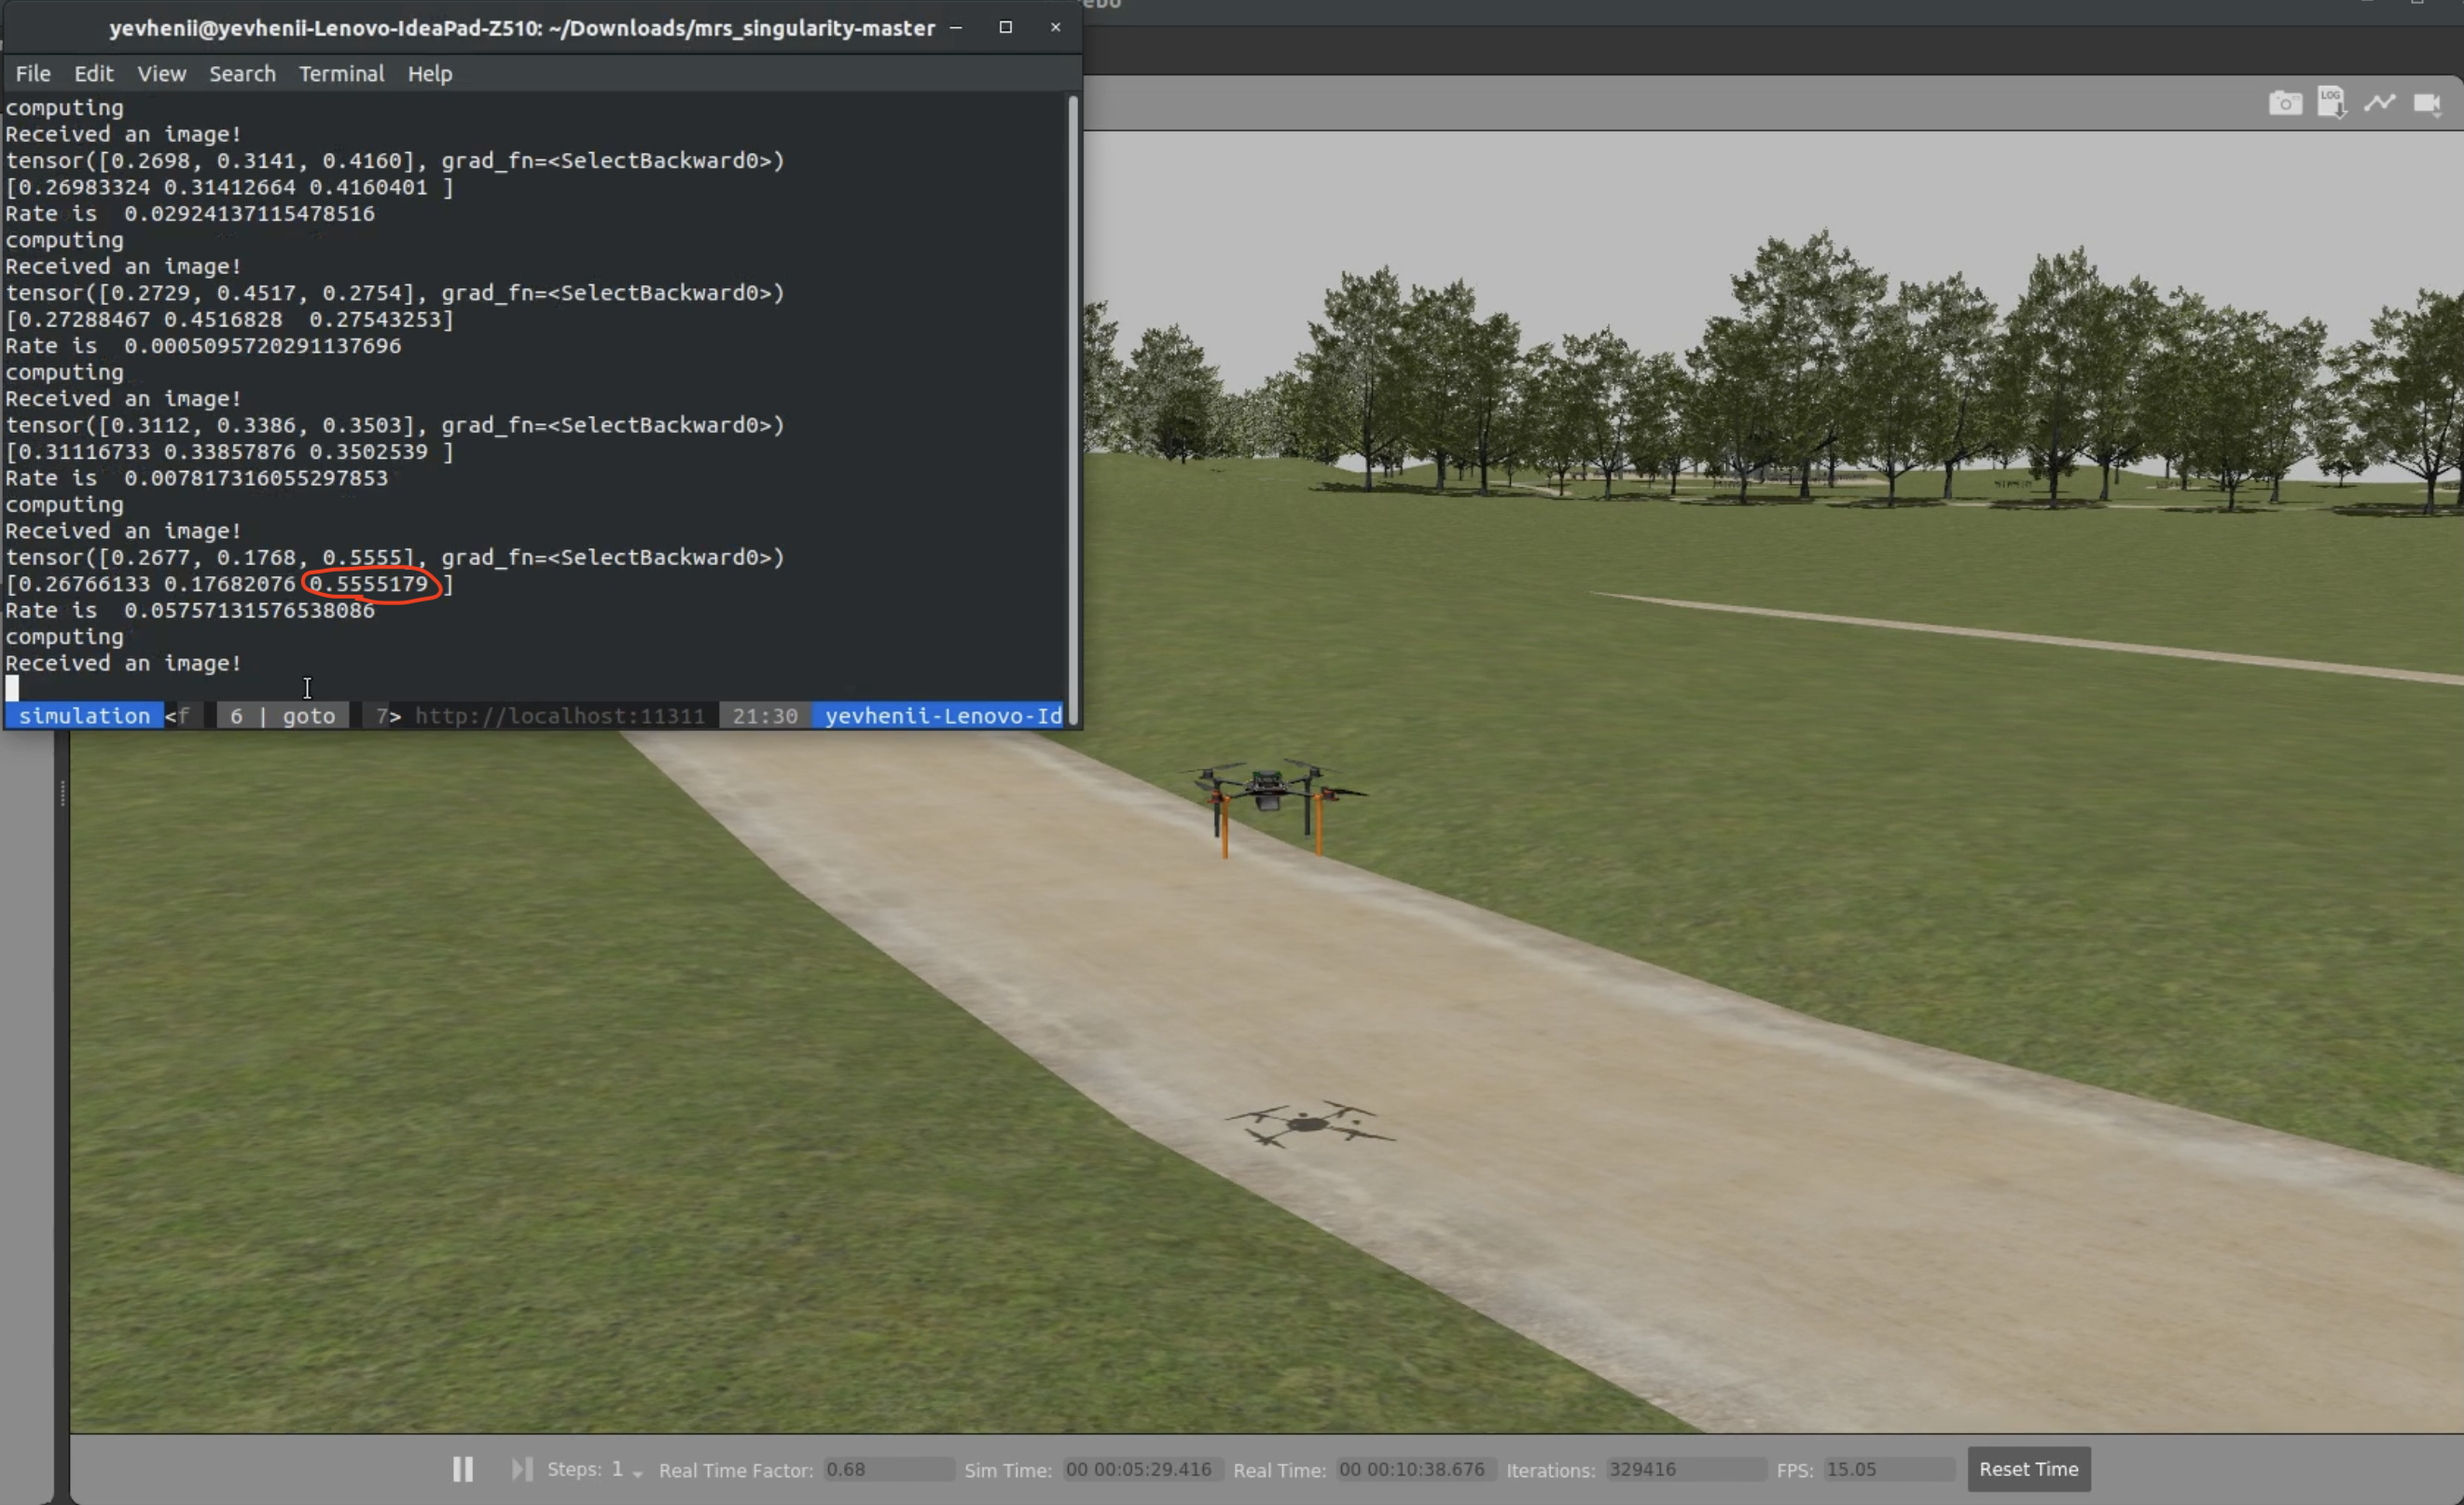
\includegraphics[width=0.75\textwidth]{./fig/photos/sim_right.png}
    \label{fig:sim_right}
  }

  \centering	
  

  \subfloat[Prediction "straight" is most likely, \acs{UAV} is pointed straight. Vehicle moves forward.] {
    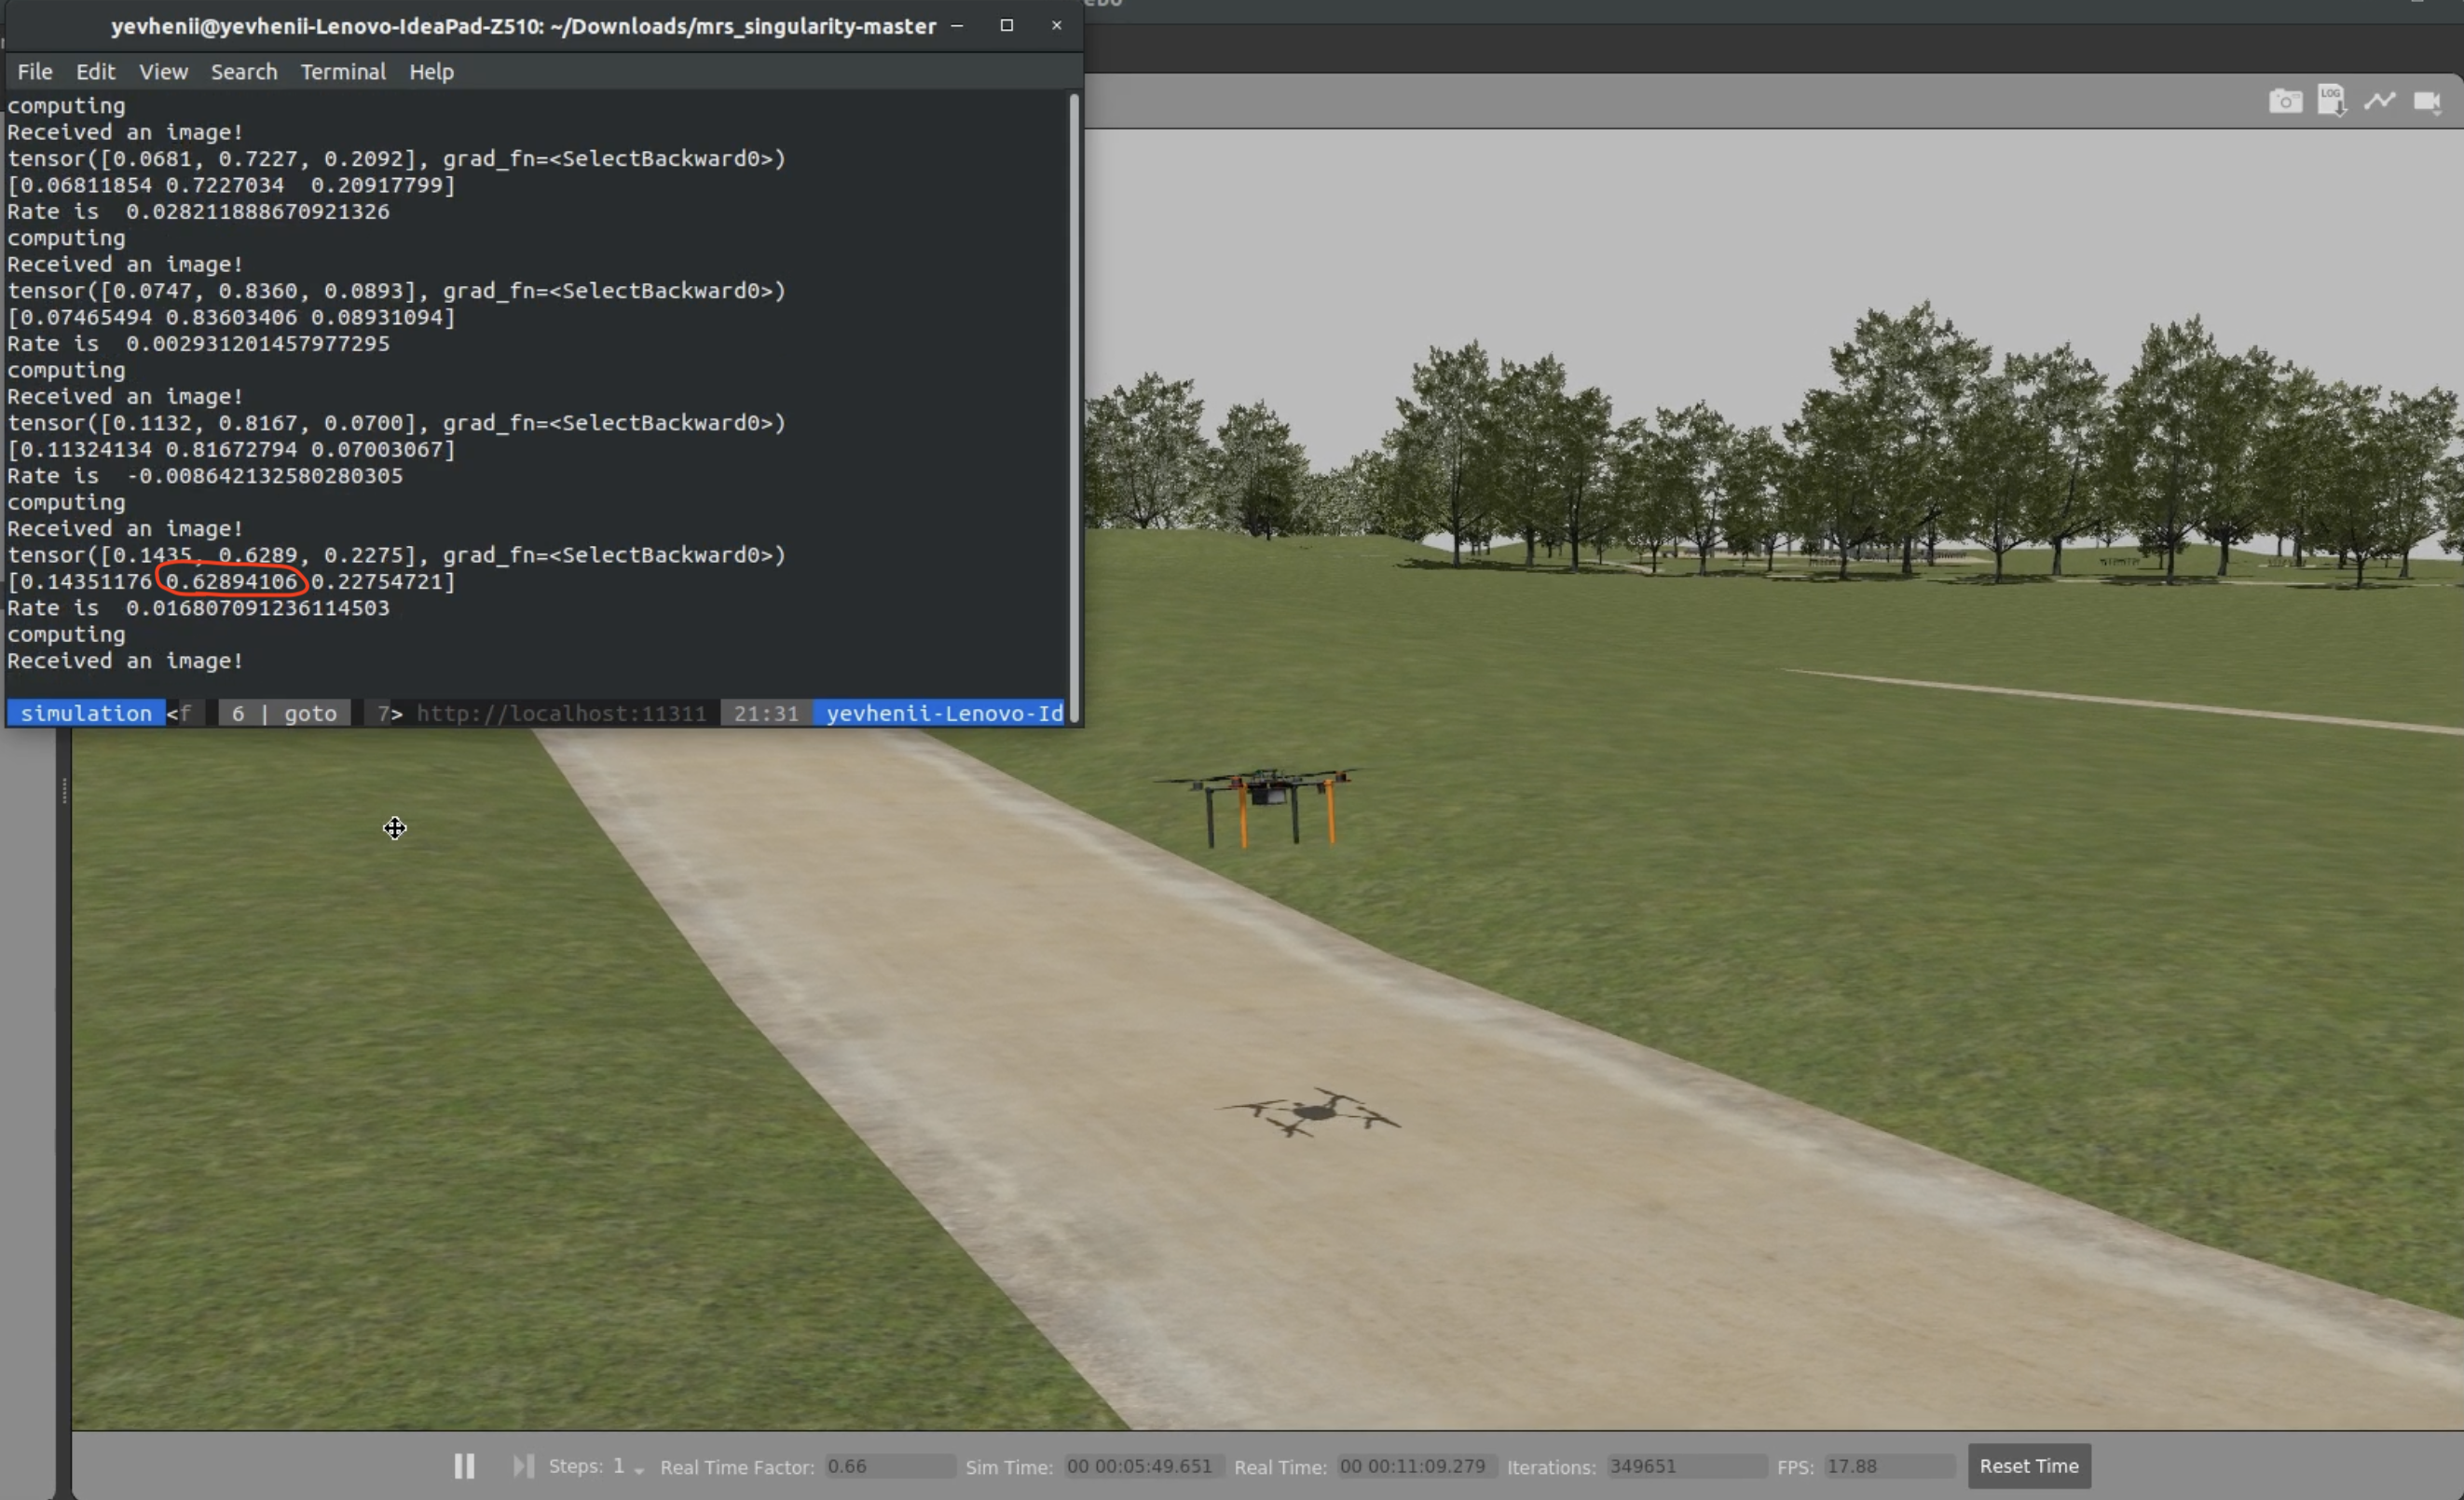
\includegraphics[width=0.75\textwidth]{./fig/photos/sim_straight.png}
    \label{fig:sim_straight}
  }

  \caption{Predictions during simulation.}
  \label{fig:sim}
\end{figure}







\chapter{Experiment}

\section{Neural network performance test}

For evaluation of the neural network performance in real-world forest conditions I decided to take a walk with the on-board computer and the camera, all powered from  the battery. Data was outputed in real-time to my laptop and I was able to evaluate the prediction correctness (\reffig{fig:test_nn}).


\begin{figure}[!h]
  \begin{minipage}{.5\linewidth}
  \centering
  \subfloat[Camera pointed straight.] {
    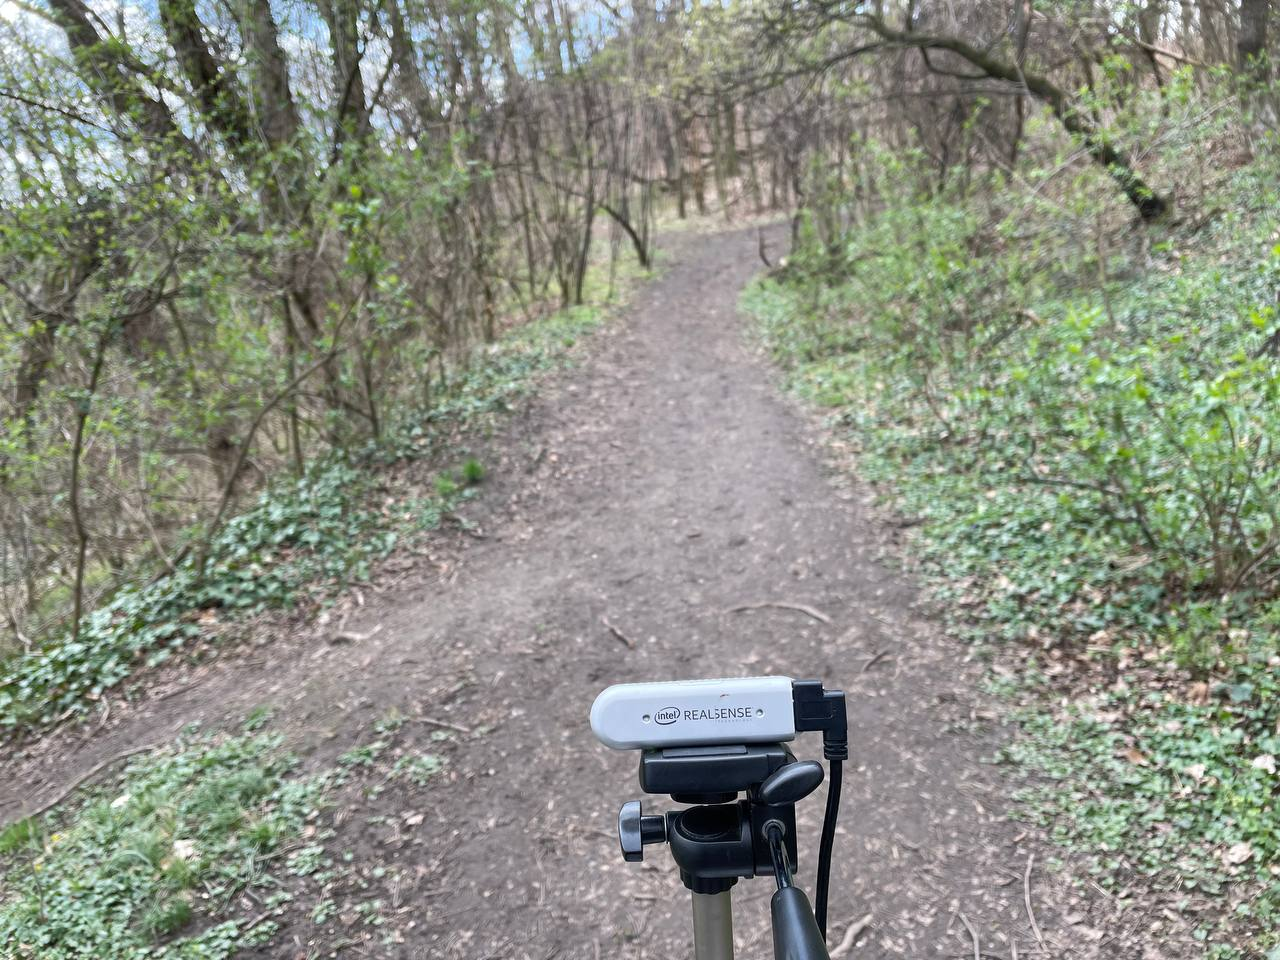
\includegraphics[width=0.9\textwidth]{./fig/photos/nn_1_1.jpg}
    \label{fig:nn_1_1}
  }
  \end{minipage}
  \begin{minipage}{.5\linewidth}
  \centering	
  

  \subfloat[Prediction: "straight" is most likely.] {
    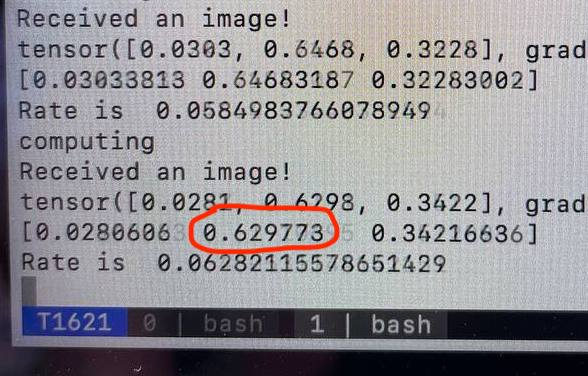
\includegraphics[width=0.9\textwidth]{./fig/photos/nn_2_1.jpg}
    \label{fig:nn_2_1}
  }
  \end{minipage}
  
  
  \begin{minipage}{.5\linewidth}
  \centering
  \subfloat[Camera is pointed left.] {
    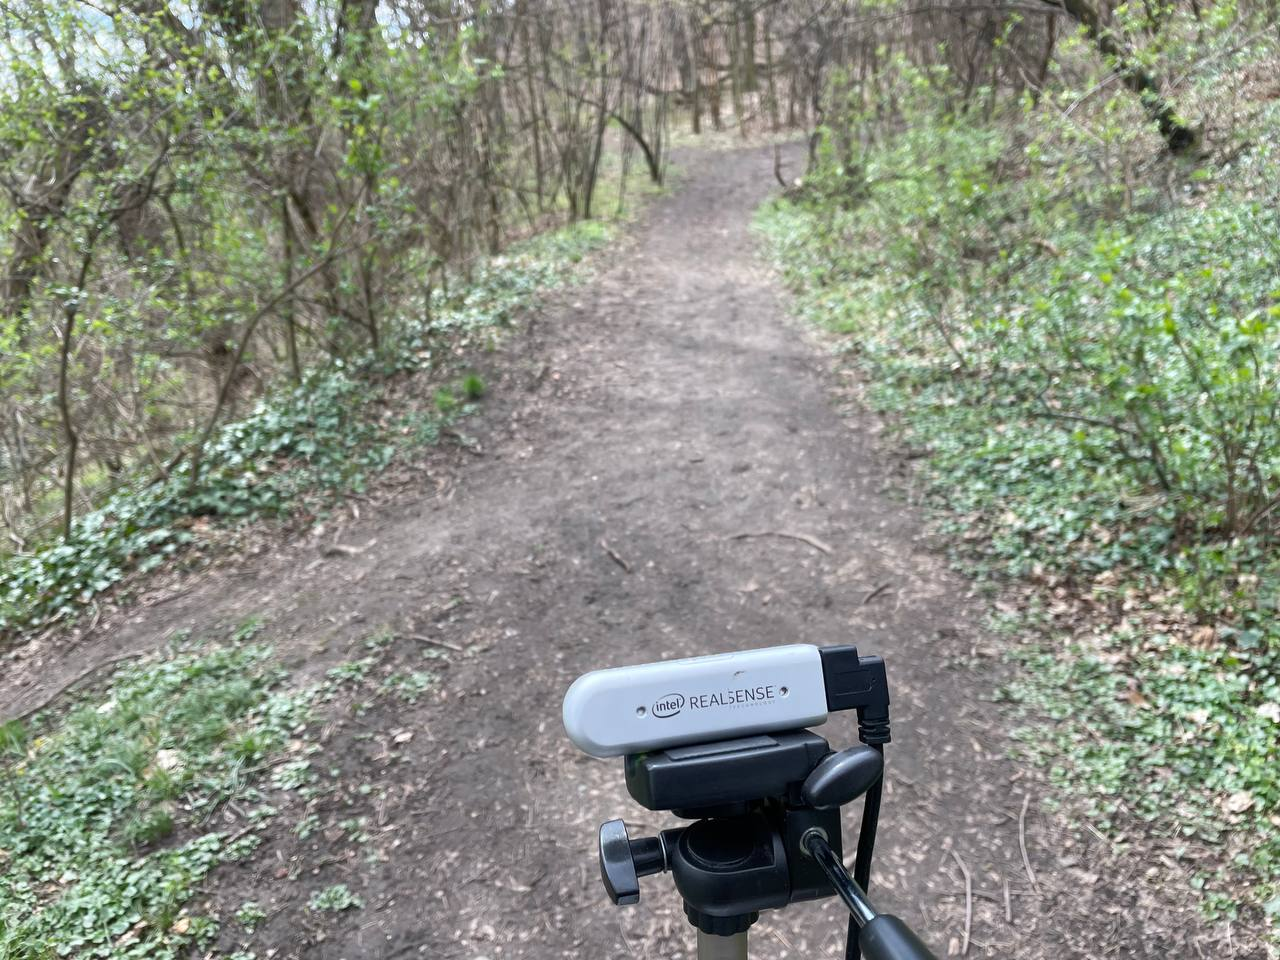
\includegraphics[width=0.9\textwidth]{./fig/photos/nn_1_2.jpg}
    \label{fig:nn_1_2}
  }
  \end{minipage}
  \begin{minipage}{.5\linewidth}
  \centering	
  

  \subfloat[Prediction: "left" is most likely.] {
    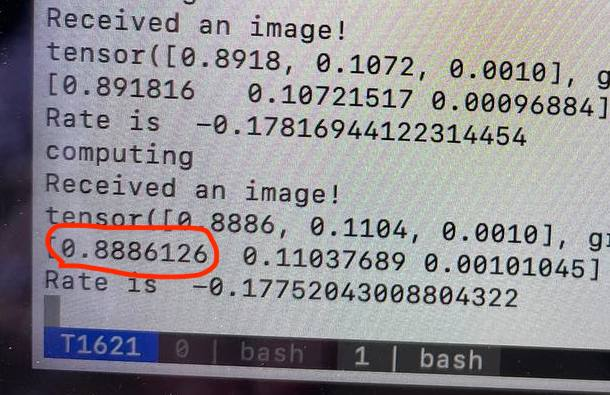
\includegraphics[width=0.9\textwidth]{./fig/photos/nn_2_2.jpg}
    \label{fig:nn_2_2}
  }
  \end{minipage}
  
  \begin{minipage}{.5\linewidth}
  \centering
  \subfloat[Camera is pointed right.] {
    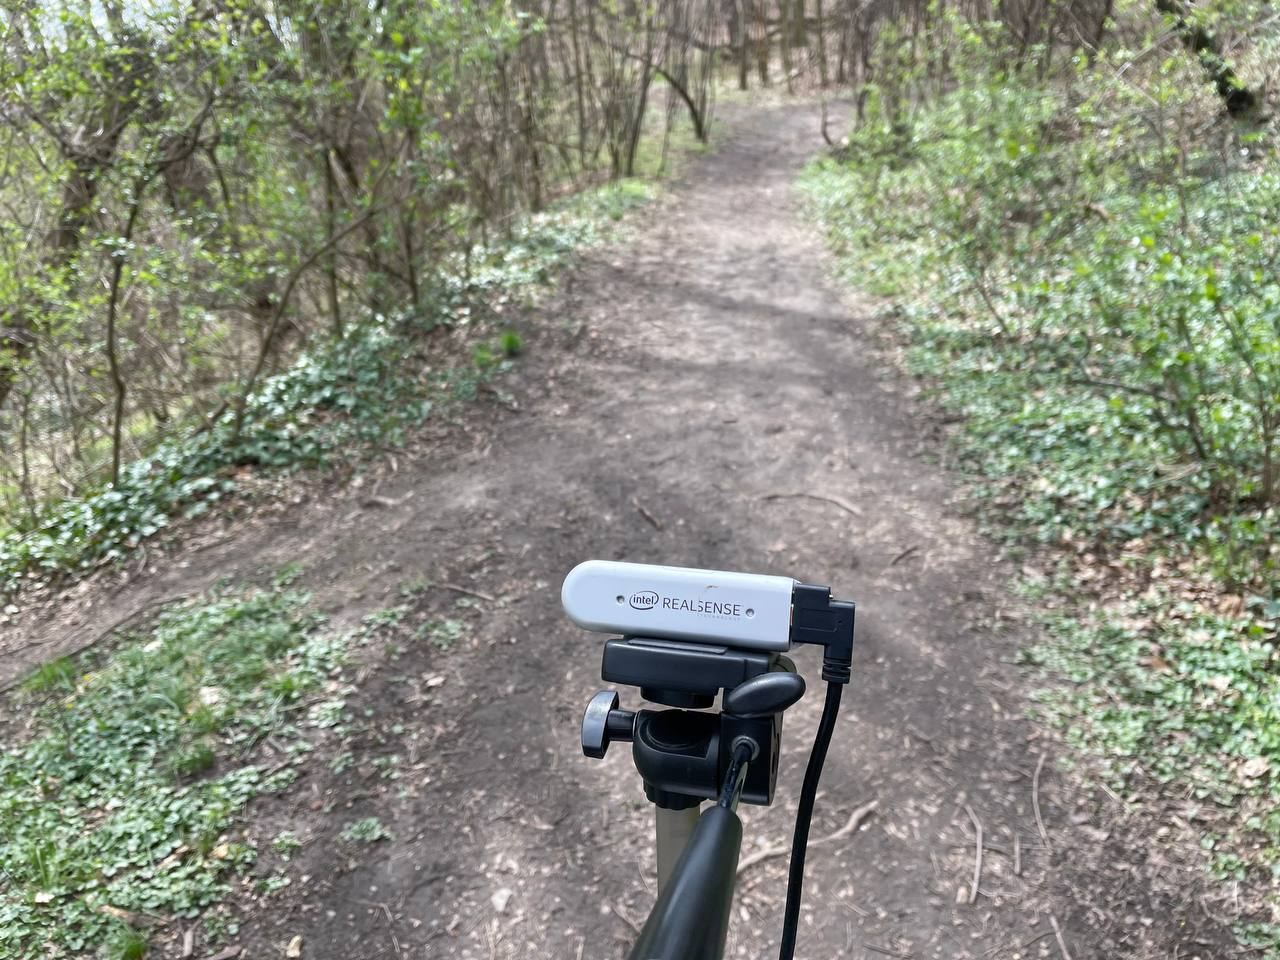
\includegraphics[width=0.9\textwidth]{./fig/photos/nn_1_3.jpg}
    \label{fig:nn_1_3}
  }
  \end{minipage}
  \begin{minipage}{.5\linewidth}
  \centering	
  

  \subfloat[Prediction: "right" is most likely.] {
    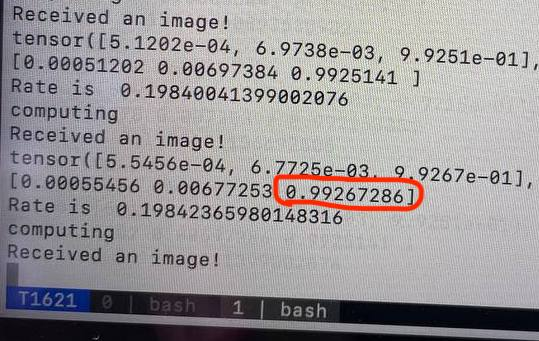
\includegraphics[width=0.9\textwidth]{./fig/photos/nn_2_3.jpg}
    \label{fig:nn_2_3}
  }
  \end{minipage}
  
  
  \caption{Neural network performance test.}
  \label{fig:test_nn}
\end{figure}

Testing showed good neural network performance. Accuracy of determining the "left" and "right" classes in situation where it is also possible for humans was 100\%. There was once a situation though, where the neural network was outputting small probability of "straight" class, when looking straight. Probabilities of "left" and "right" were same, close to 50\%. But the issue was clearly dependent on the tilt angle of a camera, after tilting it a few degrees down, problem was solved. Possible source of issue could be not only the neural network fail-case, but also lens flare.

\section{Complete tests on vehicle}

Real-world evaluation was conducted in a forest near the Czech town Temešvár. Together with \acs{MRS} team, we have found a suitable forest trails, where an algorithm can be thoroughly tested. Trails are of different complexity (visually) and contain slight obstacles on the sides (\reffig{fig:trails}). 

\begin{figure}[!h]

  \centering
  \subfloat[Trail 1.] {
    \includegraphics[width=0.72\textwidth]{./fig/photos/path_1_op.png}
    \label{fig:path_1}
  }

  \centering	
  

  \subfloat[Trail 2.] {
    \includegraphics[width=0.72\textwidth]{./fig/photos/path_2_op.png}
    \label{fig:path_2}
  }

  \centering
  \subfloat[Trail 3.] {
    \includegraphics[width=0.72\textwidth]{./fig/photos/path_3_op.png}
    \label{fig:path_3}
  }
  \caption{Three trails used for testing}
  \label{fig:trails}
\end{figure}

First trail (\reffig{fig:path_1}) is a partly dirty asphalt road with turns, surrounded by trees and bushes, 2.3\,m wide. The \acs{UAV} travelled approximately 80 meters through this road. Due to the limited \acs{FOV} of the camera and relatively wide trail, when being in the middle of it, vehicle was seeing only a grey dull pattern with no features and because of that outputed 100\% probability of "straight" class even when not pointed straight. But as soon as the \acs{UAV} gets close to the road edge, neural network recognises it and gives the command to turn in opposite direction. Then it starts flying along the path and slowly getting closer to the other side and same situation happens. However, this "zig-zag" behaviour does not affect the performance too much. But in some situations flying close to the road edge is dangerous and during this test, path planner prevented the vehicle from executing several waypoints due to their proximity to an obstacle (\reffig{fig:avoid_1}). Problem can be solved by using a camera with wider \acs{FOV}. Travelled distance on the first path is 130\,m (\reffig{fig:satellite_1}).

TODO: images from the drone with probabilities and point cloud

\begin{figure}[!h]

  \centering
  \subfloat[\acs{UAV} avoiding an obstacle.] {
    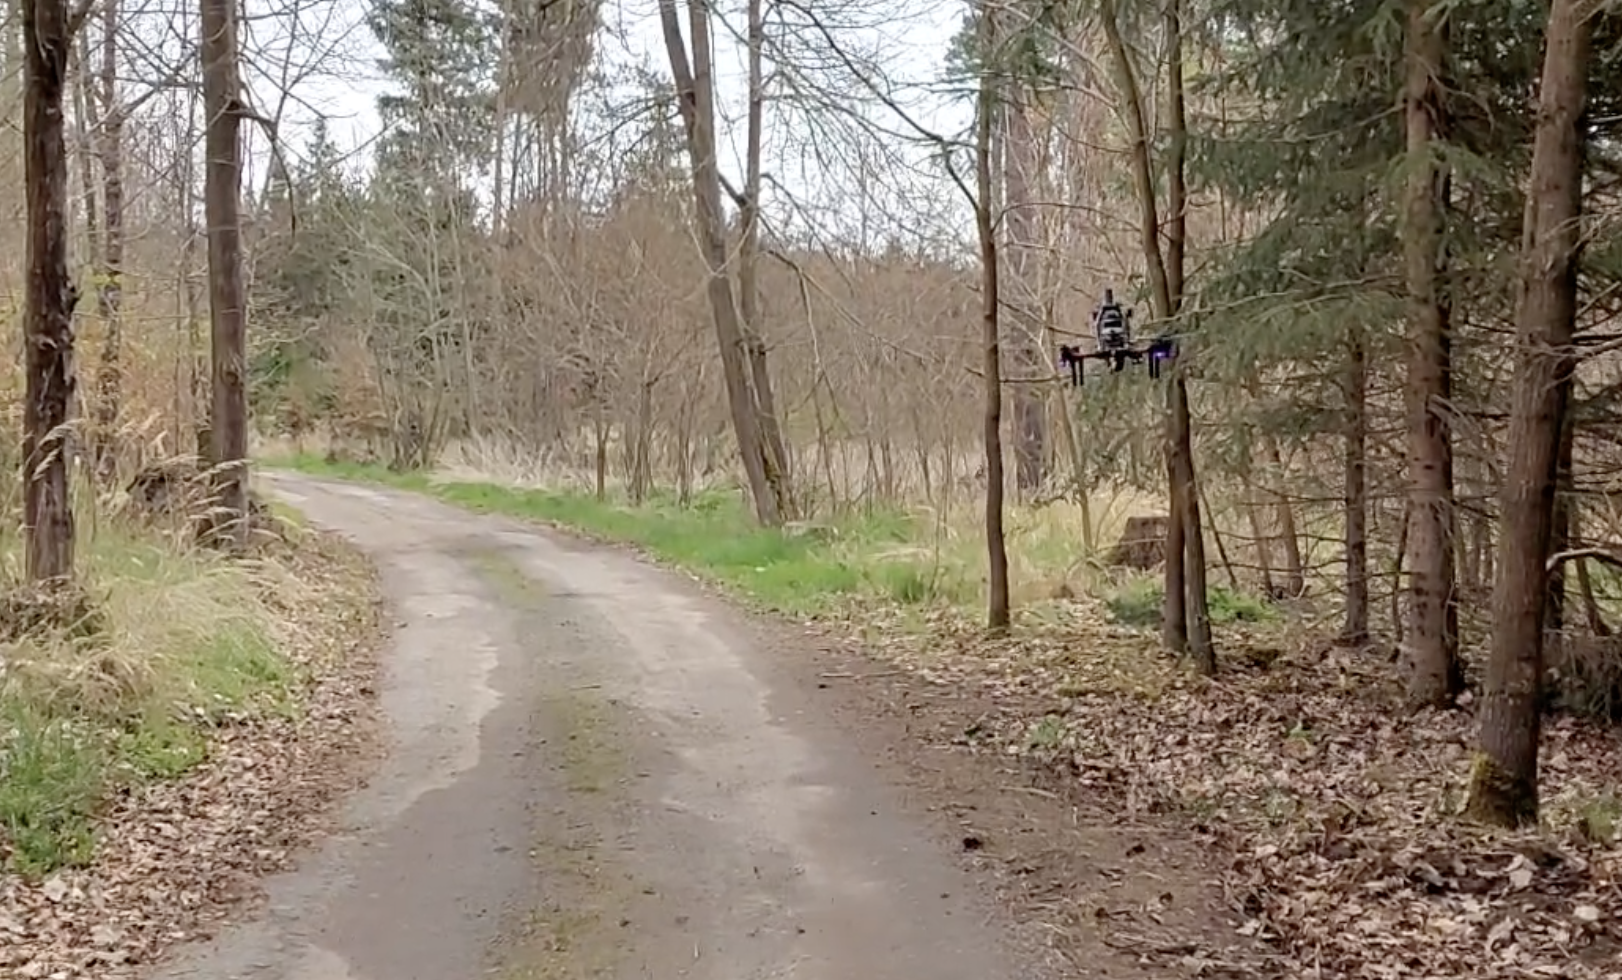
\includegraphics[width=0.72\textwidth]{./fig/photos/path_1_avoid.png}
    \label{fig:avoid_1}
  }

  \centering	
  

  \subfloat[Satellite image.] {
    \includegraphics[width=0.72\textwidth]{./fig/photos/path_1.png}
    \label{fig:satellite_1}
  }

  \caption{First experiment.}
  \label{fig:first_trail_photos}
\end{figure}


Second trail (\reffig{fig:path_2}) is a completely dirt road 2-2.3\,m wide with one sharp turn and fences on sides. It was hard for the \acs{UAV} to stay on it. A lot of distractive features were present on the road and trail itself was not well maintained. When analysing the images, it can be seen that contrast between the trail and dry grass on sides is very low. Probably, colour adjustments of the camera are required and also including such low-contrast images to the dataset should help. Also, there was a ditch on the road which looked like a trail for the \acs{UAV} (\reffig{fig:confused_2}). However, when obstacle avoidance prevented it from flying into the bush, real trail reappeared in the field of view and vehicle managed to return on track. At the end, it got distracted again. Such trail was not followed with much success, but after mentioned improvements, results should be way better. Total travelled distance on this path was 40\,m (\reffig{fig:satellite_2}).

TODO: image of low contrast, onboard

\begin{figure}[!h]

  \centering
  \subfloat[\acs{UAV} got confused by a ditch, photo before recovery.] {
    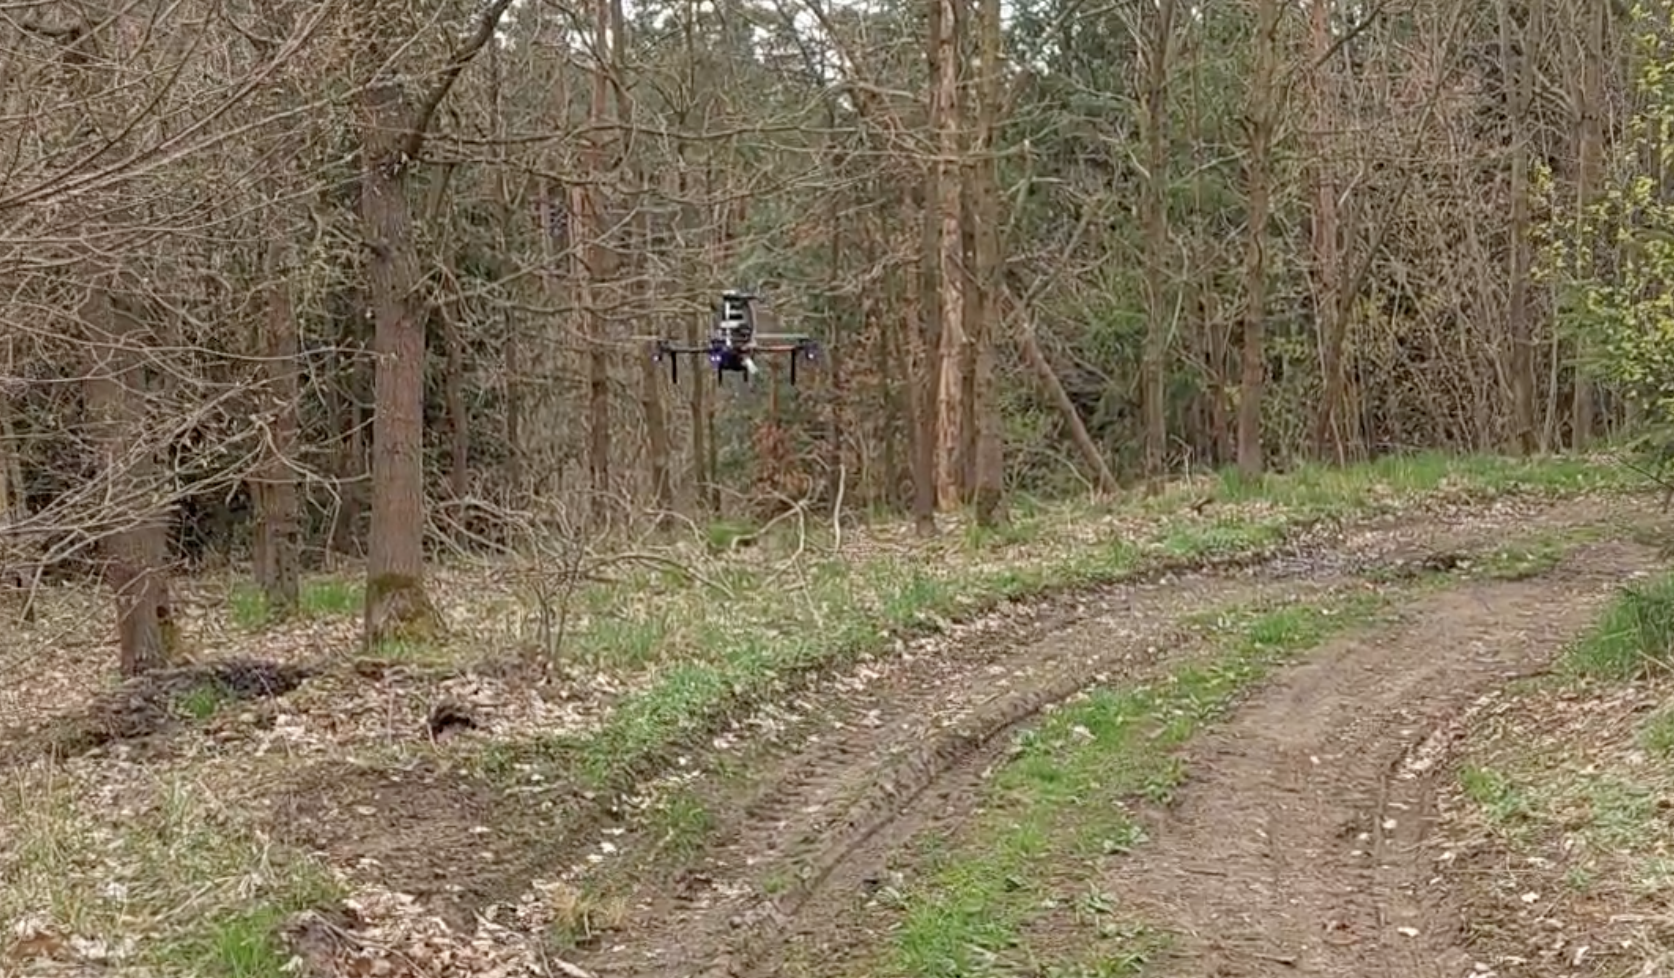
\includegraphics[width=0.72\textwidth]{./fig/photos/path_2_confused.png}
    \label{fig:confused_2}
  }

  \centering	
  

  \subfloat[Satellite image.] {
    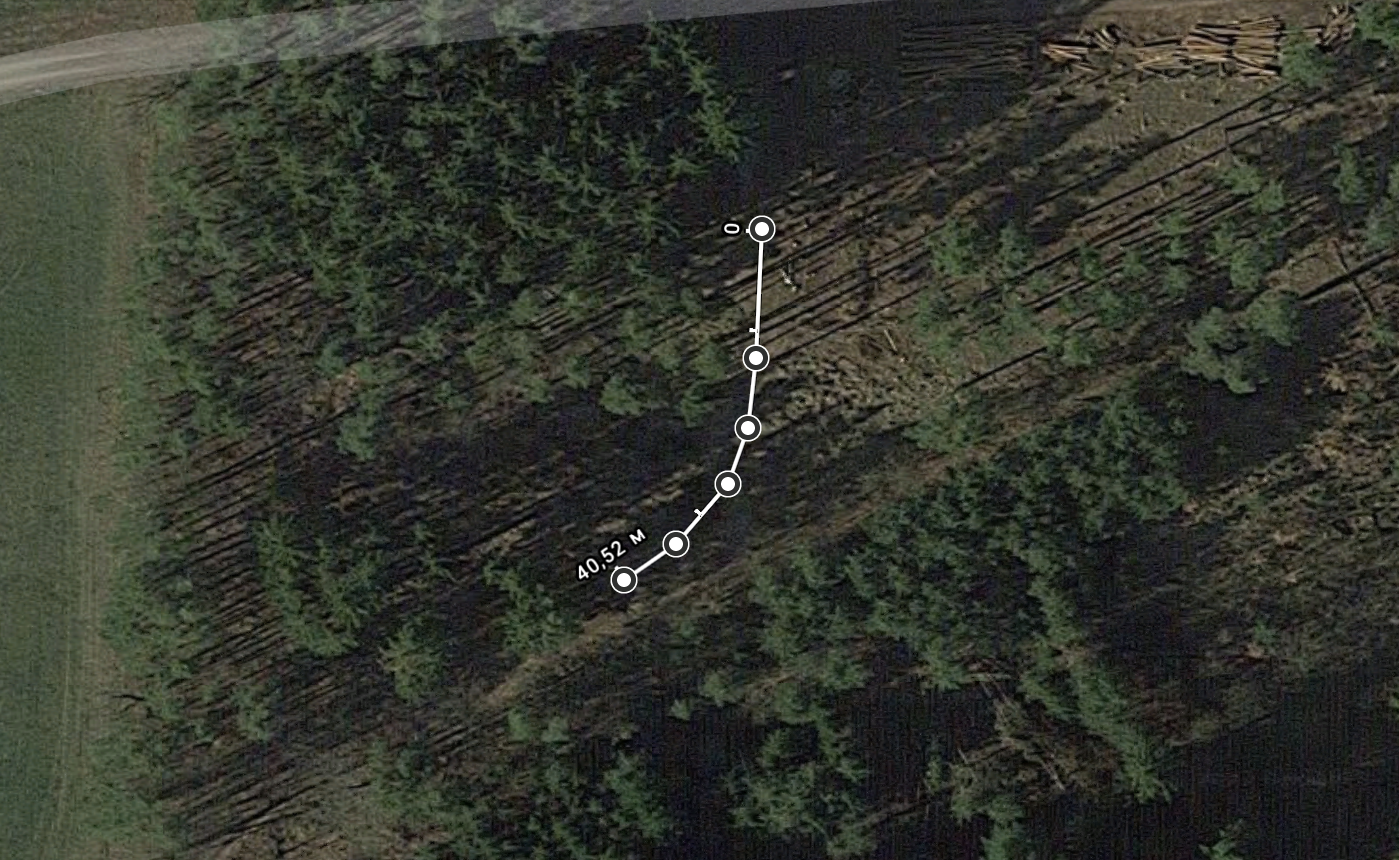
\includegraphics[width=0.72\textwidth]{./fig/photos/path_2.png}
    \label{fig:satellite_2}
  }

  \caption{Second experiment.}
  \label{fig:second_trail_photos}
\end{figure}

Third trail (\reffig{fig:path_3}) is a gravel and dirt road with slight turns. Contrast between the road and sides on the gravel part is better than on previous trails. On dirt part contrast gets much lower, distinction between trail and sides is not as clear. But it has not not confused the \acs{CNN}. Its performance was better than on other trails. \acs{UAV} has flown a long way through it. However, in the end it got confused by the lying logs and vehicle started "following" one of them (\reffig{fig:fail_log_3}). It has probably happened due to the road and sides being both covered in dirt and from vehicle camera perspective they were not distinguishable. Total path flown is 160\,m on this trail (\reffig{fig:satellite_3}).

\begin{figure}[!h]

  \centering
  \subfloat[\acs{UAV} got confused by the log.] {
    \includegraphics[width=0.72\textwidth]{./fig/photos/path_3_fail_log.png}
    \label{fig:fail_log_3}
  }

  \centering	
  

  \subfloat[Satellite image.] {
    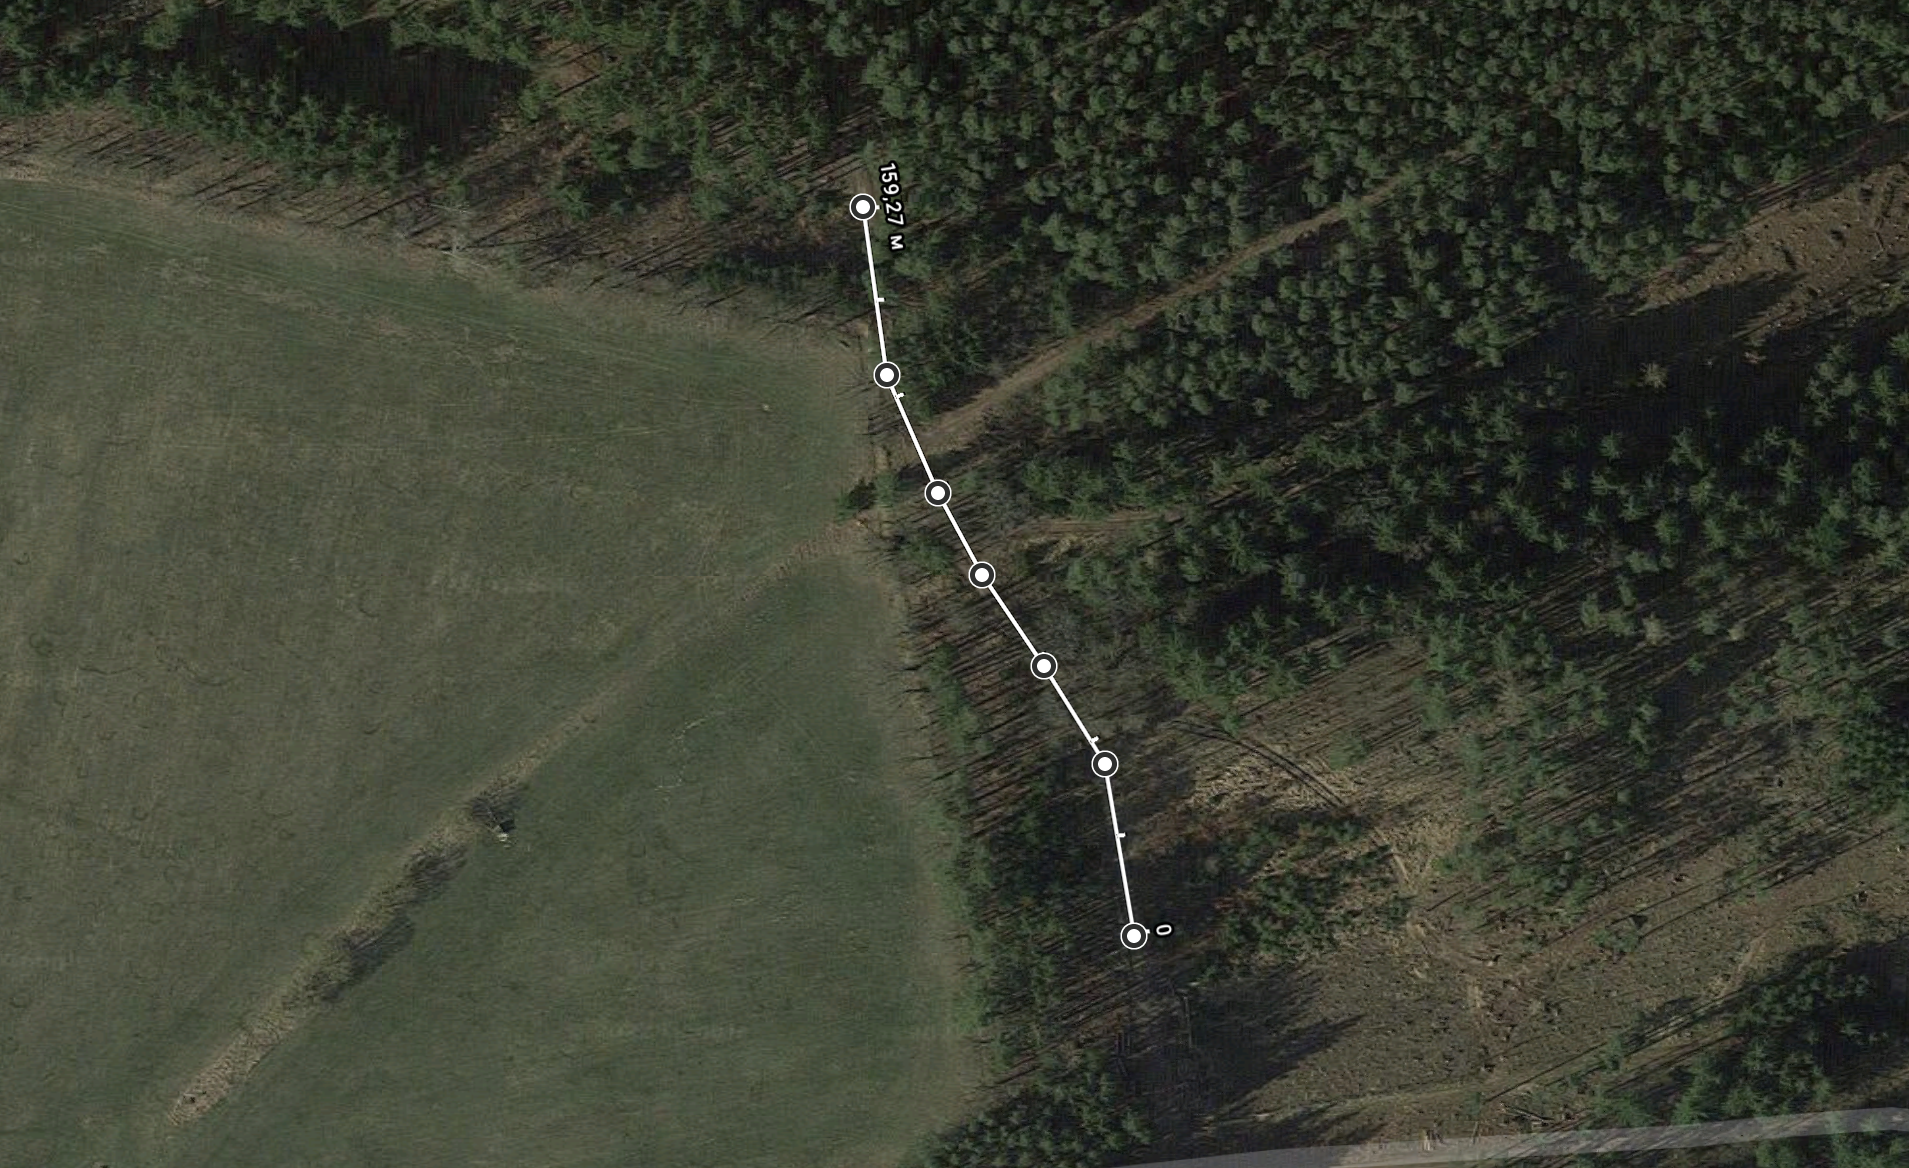
\includegraphics[width=0.72\textwidth]{./fig/photos/path_3.png}
    \label{fig:satellite_3}
  }

  \caption{Third experiment.}
  \label{fig:third_trail_photos}
\end{figure}


\chapter{Conclusion}


In this thesis, a classification convolutional neural network was implemented to solve the trail following problem utilising purely visual approach. Using only an RGB camera is a cheap solution and no other hardware than onboard PC with camera is mandatory to run the program. Also, neural network is supplemented by an algorithm, which generates trajectory points according to prediction. Program is able to run in Gazebo simulations and in real-world conditions online and was tested in both virtual and real environments. 

During the training process, neural network showed up to 90\% accuracy on validation dataset. However, this dataset was acquired by other cameras than those used in this thesis. During the experiments, vehicle was able to fly relatively long distances on curvy trails (up to 160\,m), but got stuck when trail was not contrast enough or distracting factors appeared in the image. This problem can be caused by a different \acs{FOV} of used camera, colour rendering, image sensor quality and even season. Therefore, results can be improved by creating a new large dataset with conditions close to the expected and training the network on it. Also, increasing the field of view should help, because more features can be captured by the camera.

Another possible improvement can be usage of a segmentation neural network, it allows to predict also the shape of the future trajectory. However, it may be challenging to distinguish the road from the sides during segmentation, and requires a big manually labeled dataset. Therefore, in this thesis only classification approach was taken.

Implemented algorithm is a good base and addition for more complex navigation solutions in forest conditions. It was demonstrated during experiments, when \acs{LiDAR}-based obstacle avoidance and path planning was run alongside with trail-following neural network. It prevented the \acs{UAV} from flying too close to dangerous obstacles like trees or bushes.

Assignment of creating a ready-to-run trail-following algorithm for \acs{MRS} \acs{UAV}s was satisfied and tested with a team. Developed program showed relatively good performance. In spite of that, there is still a lot of room for improvements and tweaks, because in challenging environments a probability of failure is high.


%% |                         References                         |
%% --------------------------------------------------------------

\chapter{References}

\printbibliography[heading=none,title={}]

%% --------------------------------------------------------------
%% |                         Appendices                         |
%% --------------------------------------------------------------

\appendix
\renewcommand\chaptername{Appendix}

\renewcommand{\thechapter}{A}
\renewcommand\chaptername{Appendix A}

\chapter{Appendix A}

\end{document}
